% ****************************************************************************************** % Dissertation template and document class
% Author  : 
% ****************************************************************************************** %
%%% For print copies
%% set 'singlespace' option to set entire thesis to single space, and define "\printmode" to remove all hyperlinks for printed copies of the thesis. Delete all output files before changing this mode -- it will turn hyperref package on and off
%\newcommand{\printmode}{}

%%% For the electronic copy, use doublespacing, define "\proquestmode" to use outlined links, instead of colored links. 
\documentclass[a4paper,12pt]{pieasthesis}
\newcommand{\proquestmode}{} %\printmode or \proquestmode
\title{A Reference Book of Physics \\ Volume II}

%\submitted{October 10, 2011}  % degree conferral date (January, April, June, September, or November)
%\copyrightyear{2011}  % year in which the copyright is secured by publication of the dissertation.
\author{Assad Sultan}
%%%%%%%%%%%%%%%%%%%%%%%%%%%%%%%%%%%%%%%%%%%%%%%%%%%%%%%%%%%%%\
    \renewcommand{\topfraction}{0.85}	% max fraction of floats at top
    \renewcommand{\bottomfraction}{0.6}	% max fraction of floats at bottom
    \setcounter{topnumber}{2}
    \setcounter{bottomnumber}{2}
    \setcounter{totalnumber}{4}     % 2 may work better
    \setcounter{dbltopnumber}{2}    % for 2-column pages
    \renewcommand{\dbltopfraction}{0.66}	% fit big float above 2-col. text
    \renewcommand{\textfraction}{0.15}	% allow minimal text w. figs
    %   Parameters for FLOAT pages (not text pages):
    \renewcommand{\floatpagefraction}{0.66}	% require fuller float pages
	% N.B.: floatpagefraction MUST be less than topfraction !!
    \renewcommand{\dblfloatpagefraction}{0.66}	% require fuller float pages

\usepackage{graphicx,verbatim,amsmath,multirow,longtable,booktabs,epsfig,epstopdf,multicol}
\setlength{\LTcapwidth}{\textwidth}
\usepackage[top=1in, bottom=1in, left=1.5in, right=1in]{geometry}
%%%%%%%%%%%%%%%%%%%%%%%%%%%%%%%%%%%%%%%%%%%%%%%%%%%%%%%%%%
%%% Printed vs. online formatting
\ifdefined\printmode
% Printed copy

% url package understands urls (with proper line-breaks) without hyperlinking them
\usepackage{url}
\else
\ifdefined\proquestmode
\usepackage[hidelinks]{hyperref}
\hypersetup{bookmarksnumbered}
\makeatletter
\hypersetup{pdftitle=\@title,pdfauthor=\@author}
\makeatother

\else
\usepackage{hyperref}
\hypersetup{colorlinks,bookmarksnumbered}

% copy the already-set title and author to use in the pdf properties
\makeatletter
\hypersetup{pdftitle=\@title,pdfauthor=\@author}
\makeatother

% make the page number rather than the text be the link for ToC entries
%\hypersetup{linktocpage}
\fi % proquest or online formatting
\fi % printed or online formatting
\usepackage{sectsty}
\usepackage[english]{babel}
\usepackage[utf8x]{inputenc}
\usepackage{esvect}
\usepackage{fullpage}
\usepackage{amssymb}
\usepackage{xcolor}
\usepackage{textgreek}
\usepackage{enumitem}
\usepackage{wrapfig}
\usepackage{caption}
\usepackage{float}
\usepackage{fixltx2e}
\usepackage{listings}
\usepackage{subcaption}
\usepackage{xpatch}
%\renewcommand{\labelitemi}{$\blacksquare$}
\definecolor{subsectioncolor}{RGB}{0,73,140}
\definecolor{subsubsectioncolor}{RGB}{0,73,120}
\definecolor{paragraphcolor}{RGB}{0,73,110}
\definecolor{backgroundcheckpoint}{RGB}{204,229,255}
\definecolor{backgroundeqn}{RGB}{255,229,204}

\subsectionfont{\sffamily\itshape\color{subsectioncolor}}
\subsubsectionfont{\sffamily\color{subsubsectioncolor}}
\sectionfont{\sffamily\color{cyan}\large}
\paragraphfont{\sffamily\color{paragraphcolor}}


%\setcounter{secnumdepth}{3} 
% \setcounter{tocdepth}{3}
\setcounter{chapter}{10}
%%%%%%%%%%%%%%%%%%%%%%%%%%%%%%%%%%%%%%%%%%%%%%%%%%%%%%%%%%%%%\

\newenvironment{indenttext}{
    \begin{list}{}{ \itemsep 0in \itemindent 0in
    \labelsep 0in \labelwidth 0in
    \listparindent 0in
    \topsep 0in \partopsep 0in \parskip 0in \parsep 0in
    \leftmargin 1em \rightmargin 0in
    \raggedright
    }
    \item
  }
  {\end{list}}

% another environment that's an indented list, with no spaces between items -- if we want multiple items/lines. Useful in tables. Use \item inside the environment.
% 	\raggedright makes them left aligned instead of justified
\newenvironment{indentlist}{
    \begin{list}{}{ \itemsep 0in \itemindent 0in
    \labelsep 0in \labelwidth 0in
    \listparindent 0in
    \topsep 0in \partopsep 0in \parskip 0in \parsep 0in
    \leftmargin 1em \rightmargin 0in
    \raggedright
    }

  }
  {\end{list}}
  \ifodd 0
  % you can just skip the \acknowledgements and \dedication commands to leave out these sections.
  \else
  \dedication{Dedicated to our Parents for their love and affection}
  % \acknowledgements{
  % \chapter*{Acknowledgements}
\addcontentsline{toc}{chapter}{Acknowledgements}

I would like to thank the Math department for providing the original documentclass file that this class is based upon. I would like to thank my parents, without whom my life would not be possible. I would also like to thank my advisor, my dissertation committee, and my research collaborators because every graduate student needs to do so. And finally, I thank the members of my research group, to whom I leave this template to save you some of the trouble I had to go through getting my dissertation to compile in \LaTeX{}.  

Don't forget to ask your advisor if your work was sponsored by a grant that needs to be acknowledged in this section.  
  % }
  \abstract{
  \chapter*{Abstract}
\addcontentsline{toc}{chapter}{Abstract}
The property of a physical system by which the response to an applied force is delayed in its e?ect, is referred to as time-delay. Physical transmission of material, information or energy from one place to another, is always associated with time-delay. The size of delay is determined by the distance and the transmission speed. Some delays are short, some are very long. The presence of long delays makes system analysis and control design much more complex. What is worse is that some delays are too long to perceive and the system is misperceived as one without delays.
  }


\usepackage{fancyhdr}
\pagestyle{fancy}
\renewcommand{\chaptermark}[1]{\markboth{\normalfont\thechapter.\space#1}{}}
\newcommand{\schaptermark}[1]{\markboth{\normalfont#1}{}}
\makeatletter

\def\@schapter#1{\if@twocolumn
\@topnewpage[\@makeschapterhead{#1}]
\else
\@makeschapterhead{#1}%
\schaptermark{#1}%
\@afterheading
\fi}
\makeatother

\fancypagestyle{plain}{
  \fancyhf{} % clear all header and footer fields
  \fancyhead[R]{\nouppercase{\leftmark}}
  \fancyhead[L]{A Reference Book of Physics, Vol II}
  \fancyfoot[R]{\thepage}
  \renewcommand{\plainheadrulewidth}{0.5pt} 
  \renewcommand{\plainfootrulewidth}{0pt}
}
\fancyhf{}
\fancyhf{} % clear all header and footer fields
\fancyhead[R]{\nouppercase{\leftmark}}
\fancyhead[L]{A Reference Book of Physics, Vol II}
\fancyfoot[R]{\thepage}
\renewcommand{\headrulewidth}{0.5pt} 
\renewcommand{\footrulewidth}{0pt}

\renewcommand{\footnoterule}{%
\kern -3pt
\hrule width \textwidth height 1pt
\kern 2pt 
}
\usepackage[titletoc]{appendix}
\setlength{\headsep}{10pt}

\usepackage{tcolorbox}
% \tcbset{
%   frame code = {},
%   center = title,
%   left = 0pt,
%   right = 0pt,
%   top = 0pt,
%   bottom = 0 pt,
%   colback = backgroundcheckpoint,
%   colframe = white,
%   width = \dimexpr\textwidth\relax,
%   enlarge left by = 0mm,
%   boxsep = 5pt,
%   arc = 0pt, outer arc = 0pt,
% }

\newtcolorbox{mybox}[3][]
{
  colframe = #2!25,
  colback = #2!10,
  coltitle = #2!20!black,
  title = {#3},
  #1,
  %boxsep = 5pt,
}
\usepackage{scalerel}
\def\capacitor{\scalerel*{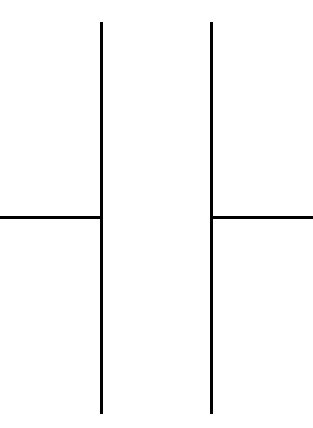
\includegraphics{Images/capacitor}}{X}}%
\def\checkpoint{\scalerel*{
\includegraphics{Images/checkpoint}}{X}}
\def\note{\scalerel*{
\includegraphics{Images/Note}}{X}}
\def\resistor{\scalerel*{
\includegraphics{Images/resistor}}{X}}
% \newcommand{\checkpoint}
% {
%     {
\includegraphics[height = 1.5em]{Images/checkpoint.png}}
% }
\begin{document}

\makefrontmatter
\chapter{Electrostatics}
\label{11}
\section{Electric Charge}
\textit{``Electric charge is a basic property of elementary particles that causes them to exert forces on one another.”}\\
\indent Alternatively, we can define electric charge as, \textit{“A physical quantity whose presence produces an electric field.”}
\subsection*{Explanation}
Charge is a fundamental property of some elementary particles like 
electron, proton etc. There are two kind of charges; positive and 
negative. Protons are present inside the nucleus of an atom, possess 
positive charge and electrons are clouding around the nucleus of an 
atom, carry negative charge. All protons are alike and have the same 
charge +e = 1.60219$\times$10\textsuperscript{-19} coulomb. Similarly all electrons are alike 
and have the same charge -e. e is the fundamental charge.
\subsection{Properties of Electric charge}
\subsubsection{Electrification}
``Electrification is the process in which a neutral body is 
charged by the removal or addition of electrons."

In nature, majority objects are in neutral state because the number of electrons 
is equal to the number of protons in them. If electrons are removed, a positive charge appears on the body. Similarly, if electrons are added, a negative charge 
appears on the body. It is important to note that during 
the process, charge can never be created nor destroyed.
\subsubsection{Conservation of Electric charge}
Conservation of charge means that, ``Charge can never be created nor destroyed in a process." We can 
also state it as, ``the total charge of an isolated system remains conserved."
\subsubsection{Quantization of Electric charge}
Another very basic property of electric charge is that charge is quantized. Quantization of charge means that it exists in discrete packets rather than in continuous amounts. It means that charge on a certain body can be developed due to addition or removal of one or two or three or ‘n’ electrons. Any charge q, no matter what is its origin, is an integral multiple of the 
minimum elementary charge e. Mathematically,'q' charge on a body can be expressed as:
\begin{equation*}
  q=ne \quad \textrm{and n = 1, 2, 3, …}
\end{equation*}
\subsection*{Checkpoint 11.1}
We say that charge always exists in an integral multiple of ‘e’ but we also believe in the existence of quarks 
(having charge 2/3 e, 1/3 e etc.). How is this possible?
(Answers of checkpoints are given at the end of the part).
\subsubsection{Action between Two Charges}
It has been experimentally proved that like 
charges repel each other and unlike charges do attract. This means 
that a positive charge will repel a positive and so does a negative. And positive 
attracts a negative one and a negative does attract a positive one.

\subsection*{Sciences of Electric Charges}
On the basis of state of rest or motion of electric charges, science 
of charges is divided into two branches i.e. electrostatics and 
electrodynamics.
\begin{itemize}
\item{\textbf{Electrostatics/Static Electricity:}}\\
``It is the study of electric charges at rest". 
In this chapter, we will deal with this branch. We will 
study some basic laws like Coulomb’s law, Gauss’s law etc, and 
some fundamental concepts electric field, electric potential 
and further capacitors and their related concepts.
\item{\textbf{Electrodynamics/Current Electricity:}}\\
``It is the study of electric charges in motion." We will encounter 
this in next chapter. We will study some basic concepts of current 
flow, resistance and laws like Ohm’s law and Kirchoff’s laws.
\end{itemize}

\section{Coulomb’s law}


\subsection*{Background}
As we know that electric charges attract or repel each other. To quantify
this attaraction or repulsion, Charles-Augustin de Coulomb\footnote{\textbf{\textit{Charles Augustin de Coulomb (1736 – 1806):}} Coulomb,
a French physicist, began his career as a military engineer in the West Indies.
In 1776, here turned to Paris and retired to a small estate to do his
scientific research. He invented a torsion balance to measure the
quantity of a force and used it for determination of forces of electric
attraction or repulsion between small charged spheres. He thus arrived in
1785 at the inverse square law relation, now known as Coulomb’s law. The
law had been anticipated by Priestley and also by Cavendish earlier, though Cavendish
never published his results. Coulomb also found the
inverse square law of force between unlike and like magnetic poles.},
in 1785, first measured the force of interaction (attraction or repulsion) between 
electric charges and deduced the law that governs them, called as Coulomb’s law. He used 
for this purpose an apparatus called Torsion’s balance.


\subsection*{Statement:}
``Two stationary point\footnote{As word point suggests an entity 
of no dimension.In practice,two charges are said to be point 
charges if their dimesions (means their radii) are very very smaller as compared to 
the distance between them. Coloumb’s law
has its validity over the point charges.} charges attract or repel each 
other with a force which is directly proportional to the 
product of the magnitude of the charges and is inversely 
propotional to the square of the distance between them, and 
this force acts along the line connecting the charges."

\subsection*{Mathematical Form:}
Let us consider two electric charges `q\textsubscript{1}' and `q\textsubscript{2}' 
seperated by distance `r', these charges will exert forces on one another and this 
force according to Coulomb’s law will be:
\begin{equation}
  F \propto \frac{q_{1}q_{2}}{r^{2}} \nonumber
\end{equation}
\begin{equation} \label{eq:11.1}
  F = k \frac{q_{1}q_{2}}{r^{2}} 
\end{equation}
Where k is the constant of propotionality and 
is called `Coulomb’s constant' (we will discuss it in detail later). If r is the unit vector along the line connecting the charges, then 
Coloumb’s law expression will be written as:
\begin{equation}\label{eq:11.2}
  \vec{F} = k \frac{q_{1}q_{2}}{r^{2}} \hat{r}
\end{equation}
This is the vectorial form of Coulomb's law,which shows that force is directed along the unit verctor $\hat{r}$.
We have two charges q\textsubscript{1} and q\textsubscript{2}. If q\textsubscript{1} is considered as
source charge(the charge exerting the force) and q\textsubscript{2} is considered
as field charge (the charge experiencing the force),then the unit vector $\hat{r}$
is directed from q\textsubscript{1} to q\textsubscript{2} and vice versa.
It is important to note that the direction of force is according to source charge.
\subsection*{Attractive or Repulsive Force}
For like charges, the product q\textsubscript{1}q\textsubscript{2} is positive;
the force is repulsive and is directed away from
the source charge. For unlike charges,
the force is attractive as q\textsubscript{1}q\textsubscript{2} is negative and the force is directed
towards the source charge.
\subsection*{Constant of propotionality ‘k’}
We used the constant of propotionality ‘k’ in coulomb’s law expression.
The constant ‘k’ depends upon:
\begin{enumerate}[label=(\alph*)]
\item System of units used(in which q, r and F are measured)
\item Properties of medium surrounding the charges
\end{enumerate}
In SI units,force, charge and distance are measured in newtons,
coloumbs and metres. As far as the choice of the medium is concerned,
we start with vacuum or free space. In free space and SI units,
the constant ‘k’ is written as:
\begin{equation}\label{eq:11.3}
  k = \frac{1}{4\pi\epsilon_{o}}
\end{equation}
Where '$\epsilon$\textsubscript{o}' is an electrical constant (read as ‘epsilon not’) and called
as permittivity of free space (permittivity of a medium is the property
of the medium which determines how much that medium affects the force
between the charges).
The value of '$\epsilon$\textsubscript{o}' is measured experimentally and
is found to be 8.85$\times$10\textsuperscript{-12} C\textsuperscript{2}/Nm\textsuperscript{2} (rounded to two decimal places).
Using the value of '$\epsilon$\textsubscript{o}' in equation \ref{eq:11.3}, we get value of ‘k’ equal to
8.99$\times$10\textsuperscript{9} Nm\textsuperscript{2}/C\textsuperscript{2}.
So, in SI units and for charges placed in vacuum (or free space),
Coulomb’s law in equation \ref{eq:11.4} can be written as:
\begin{equation}\label{eq:11.4}
  \vec{F} = \frac{1}{4\pi\epsilon_{o}} \frac{q_{1}q_{2}}{r^{2}} \hat{r}
\end{equation}
And in magnitude form,
(using ‘vac’ in subscript for representation of force in vacuum):
\begin{equation}\label{eq:11.5}
  F_{vac} = \frac{1}{4\pi\epsilon_{o}} \frac{q_{1}q_{2}}{r^{2}}
\end{equation}
\subsection{Coloumb’s law in Material Media}
As the constant of propotionality ‘k’ in coulomb’s law expression depends on the medium
around the charges. Therefore, if the charges are placed in a medium
of permittivity $\epsilon$, then coloumbic force will be given by:
\begin{equation}\label{eq:11.6}
  F_{med} = \frac{1}{4\pi\epsilon} \frac{q_{1}q_{2}}{r^{2}}
\end{equation}
From equation \ref{eq:11.6}, it implies that a material medium
with high permittivity is a medium which reduces appreciably
the force between the charges compared with the vacuum. For air, $\epsilon$\textsubscript{air}
is only slightly greater than $\epsilon$\textsubscript{o} (1.006) and for many practical purposes,
is taken equal to $\epsilon$\textsubscript{o}.
In order to make force more simplified, we introduce a term relative permittivity $\epsilon$\textsubscript{r},
which is defined as, “the permittivity of a medium compared with the permittivity of vacuum.” So,
it is given by the ratio:
\begin{equation}\label{eq:11.7}
  \epsilon_{r} = \frac{\epsilon}{\epsilon_{o}}
\end{equation}
So, ‘$\epsilon$\textsubscript{r}’ is a dimensionless constant.
It is also called the dielectric constant of the medium.
For vacuum or free space, $\epsilon$\textsubscript{r} = 1,and hence $\epsilon$= $\epsilon$\textsubscript{o}.
From above equation:
\begin{equation}\label{eq:11.8}
  \epsilon = \epsilon_{o}\epsilon_{r}
\end{equation}
Putting this value in equation \ref{eq:11.6}, we get:
\begin{equation}\label{eq:11.9}
  F_{med} = \frac{1}{4\pi\epsilon_{o}\epsilon_{r}} \frac{q_{1}q_{2}}{r^{2}}
\end{equation}
Here, '$\epsilon$\textsubscript{o}' is a constant and has a fixed value.
It is important to note that the value of dielectric constant εr for any material
medium is always greater than one. So force in a mterial medium
is always less than that of vacuum. This becomes more obvious,
if we take ratio of equations (11.9) and (11.5):
\begin{equation}\label{eq:11.10}
  \frac{F_{med}}{F_{vac}} = \frac{1}{\epsilon_{r}}
\end{equation}
which gives:
\begin{equation}\label{eq:11.11}
  F_{med} = \frac{F_{vac}}{\epsilon_{r}}
\end{equation}
Since $\epsilon$\textsubscript{r} $>$ 1 for any material medium, therefore force in a medium
is less than force in vacuum for two given charges by '$\epsilon$\textsubscript{r} times'.
This equation gives us a sense that how much times force in a medium is reduced as compared with the vacuum for two charges.
The above equation can also be written as:
\begin{equation}\label{eq:11.12}
  \epsilon_{r} = \frac{F_{vac}}{F_{med}}
\end{equation}
This equation provides us with another definition of dielectric constant
i.e. \textit{``the ratio of force between two point charges placed in vacuum
to the force between the same charges when the medium surrounding
them is material medium,
is called dielectric constant/relative permittivuty of that medium."}
\subsection*{Checkpoint 11.2}
Distilled water has a dielectric constant of nearly 80.
If force between the two charges placed in vacuum is 80 N.
How much the force will be when the same charges be placed in water?
\subsection{Units of Electric Charge}
\subsubsection{SI Unit}
The S.I unit of electric charge is coulomb (C), which can be defined in a number of ways stated under.
One way of defining one coloumb charge is using Coulomb’s law
expression i.e. \textit{``The charge on a body is said to be one coulomb when it exerts
a force of 9$\times$10\textsuperscript{9} N on a similar charge at a distance
of one metre from it in vacuum."}

Alternatively, we can also define it in terms of charge of an electron.As we know that:
\begin{equation}
  charge\:of\:one\:electron = e = 1.602\times10^{-19} C \nonumber
\end{equation}
So one coloumb charge will contain 6.25$\times$10\textsuperscript{18} electrons.
Hence, one coulomb can be defined as, ``The charge of 6.25$\times$10\textsuperscript{18} electrons is said to be one coloumb."

Another way of defining one coulomb charge is in
terms of current (flowing charge) i.e. \textit{``The amount of charge that flows
through a given cross section of a wire in one second if there is a steady
current of one ampere in the wire."}
\subsubsection{Multiples}
Since coloumb is a very large unit (imagine it as the charge of 6.25$\times$10\textsuperscript{18} electrons),
so its submultiples are commonly used.

1 μC = 10\textsuperscript{-6} C, 1 nC = 10\textsuperscript{-9} C, 1 pC = 10\textsuperscript{-12} C
\subsection{Coloumb's Law and Newton's Third Law}
As we know that charges exert forces on each other,
hence coloumic force is a mutual force.
To show that the force that one charge exerts on the other is
equal in magnitude but opposite in direction to the force that
it experiences by the other charge,
let us consider two point charges (assume them to be positive for convenience).
The distance between them is r, as shown in figure \ref{fig:11.1}.
\begin{figure}[H]
  \centering
  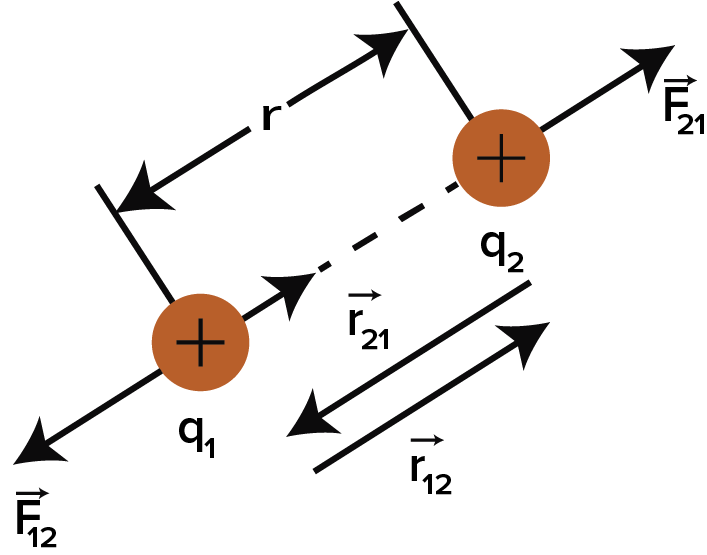
\includegraphics[scale = 0.8]{Images/11.1.png}
  \caption{Force exerted by each charge, $\vec{F_{12}}$ is the force
  exerted  on charge `q\textsubscript{1}' by `q\textsubscript{2}', $\vec{F_{21}}$ is the force exerted on charge `q\textsubscript{2}' by `q\textsubscript{1}'}
  \label{fig:11.1}
\end{figure}

Let $\vec{F_{12}}$ is the force exerted by charge `q\textsubscript{2}' on charge `q\textsubscript{1}' (subscript as, `12' means by 2 on 1)
and $\vec{r_{12}}$ is the position vector directed from `q\textsubscript{2}' to `q\textsubscript{1}'.
Similarly, $\vec{F_{21}}$  is the force exerted by charge `q\textsubscript{1}' on `q\textsubscript{2}' and  $\vec{r_{12}}$ is
the unit vector directed from `q\textsubscript{1}' to `q\textsubscript{2}'.
Since,
\begin{equation}
  \vec{r_{12}} = r_{12} \hat{r_{12}} \nonumber
\end{equation}
And,
\begin{equation}
  \vec{r_{21}} = r_{21} \hat{r_{21}} \nonumber
\end{equation}
So, $\vec{F_{12}}$ according to Coloumb's law will be given by:
\begin{equation}
  \vec{F_{12}} = k \frac{q_{1}q_{2}}{r_{21}^{2}} \hat{r_{21}} \nonumber
\end{equation}
And,
\begin{equation}
  \vec{F_{21}} = k \frac{q_{1}q_{2}}{r_{12}^{2}} \hat{r_{12}} \nonumber
\end{equation}
Since,
\begin{equation}
  \vec{r_{12}} = -\vec{r_{21}} \nonumber
\end{equation}
Therefore,
\begin{equation}
  \vec{F_{12}} = -\vec{F_{21}} \nonumber
\end{equation}
So we concluded that the force between two charges is
mutual and the forces pair is a Newton's third law pair.
\subsection{Principle of Superposition}
Coulombic force obeys the principle of superposition i.e. \textit{``The net force acting on a charge
by an assembly of charges is the vectorial
sum of all the forces exerted by the number of charges."}
\begin{figure}[H]
  \centering
  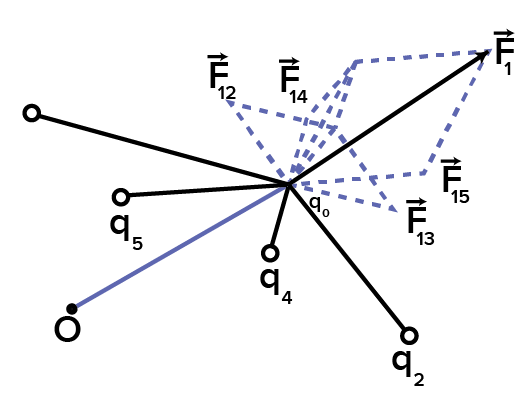
\includegraphics[scale = 1.2]{Images/11.2.png}
  \caption{Net force exerted  on charge `q\textsubscript{1}' is 
  the vectorial sum of all the forces due to each charge on `q\textsubscript{1}'.}
  \label{fig:11.2}
\end{figure}
From the figure \ref{fig:11.2}, for 'n' charges exerting a
force on the charge `q\textsubscript{1}', we can say that:
\begin{equation}  
  \vec{F_{1}} = \vec{F_{12}} + \vec{F_{13}} + \vec{F_{14}}+...+\vec{F_{1n}} \nonumber
\end{equation}
\subsection*{Checkpoint 11.3}
\begin{enumerate}[label=(\alph*)]
  \item We have two charges, `q\textsubscript{1}' and `q\textsubscript{2}'.
  Let the force of interaction between them is 4 N. Then we placed another charge `q\textsubscript{3}' in the vicinity of the charges.
  What would be the force of attraction between `q\textsubscript{1}' and `q\textsubscript{2}' now?
  \item Show that for two opposite charges, `q\textsubscript{1}' and `q\textsubscript{2}' using usual notations,
  \begin{equation}
    \vec{F_{12}} = -\vec{F_{21}} \nonumber
  \end{equation}
\end{enumerate}
\section{Electric Field and Electric Field Intensity}
\subsection*{Introduction}
The concept of electric field was introduced by \textbf{\textit{Michael Faraday}}.
He stated that the charge `q' produces an electric field surrounding it
and when a charge `q\textsubscript{o}' is brought into its field,
the field of charge `q' interacts with that of `q\textsubscript{o}' and exerts force on it.
\subsection*{Definition of Electric Field}
\textit{``The region around a charge in which a test charge
experiences an electric force, is called electric field."}
\subsection*{Explanation}
As we know that charges exert forces on each other.
Electric field is actually the region around a source charge upto
which it can exert a force on a test charge.
In order not to distort the field of a source charge,
the test charge should be small.
So the strength and direction of electric field can be determined
by placing a unit positive test charge in that field.

The strength and direction of field at a point in space is
determined by the force that a unit positive charge will
experience at that point. The direction of field is that direction
in which test charge moves or tends to move at a given point.
\subsection*{Electric Field Intensity}
\textit{``A single vector quantity containing information about the field strength and
directiom at a given point is called electric field intensity."}
\subsection*{Mathematical Form}
If `$\vec{F}$' is the force exerted on a unit positive test charge (it is a
convention to take test charge positive) `q\textsubscript{o}' by a source charge `q',
then the electric field intensity `$\vec{E}$' is given by:
\begin{equation}\label{eq:11.13}
  \vec{E} = \frac{\vec{F}}{q_{o}}
\end{equation}
Thus, it is the force per unit charge.
Defininig in this way, electric intensity is independent of test charge `q\textsubscript{o}'.
Since `q\textsubscript{o}' is always positive, therefore is always along the direction of
force on that test charge.
\subsection*{Units and Dimensions}
The S.I unit of electric field intensity is NC\textsuperscript{-1}. Another unit is volt per metre (V/m),
we will dicuss this in electric potential. Dimensions are [MLT\textsuperscript{-3}A\textsuperscript{-1}].
\subsection{Field Intensity due to a Point Charge}
In order to find an expression for field intensity due to a point charge,
consider point charges `q' and `q\textsubscript{o}' and at a distance `r' from each other.
As an example, we find the intensity of field
which exists in air around the isolated charge ‘q’.
\begin{figure}[H]
  \centering
  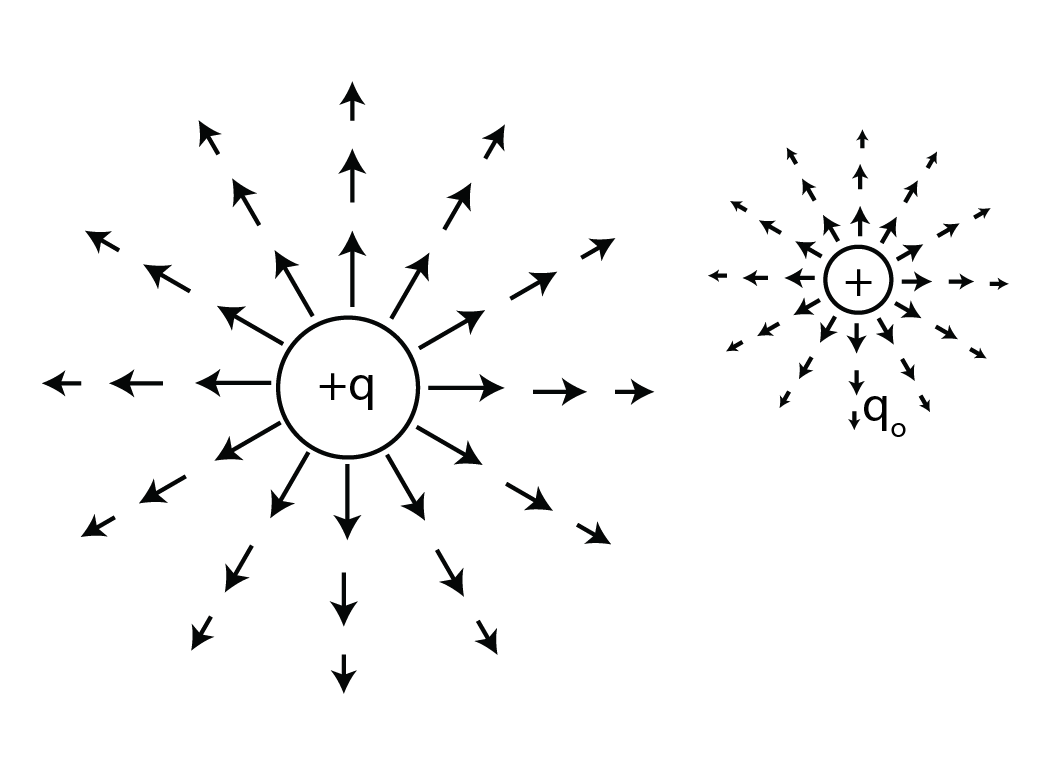
\includegraphics[scale = 0.9]{Images/11.3.png}
  \caption{Field of a source charge  `q' influencing test charge `q\textsubscript{o}'}
  \label{fig:11.3}
\end{figure}
Here `q\textsubscript{o}' is a small test charge. Coulomb’s force due
to ‘q’ on `q\textsubscript{o}' is:
\begin{equation}\label{eq:11.14}
  \vec{F} = \frac{1}{4\pi\epsilon_{o}} \frac{qq_{o}}{r^{2}} \hat{r}
\end{equation}
From the definition of electric field intensity i.e. the force per unit charge,
we can write:
\begin{equation}
  \vec{E} = \frac{\vec{F}}{q_{o}} \nonumber
\end{equation}
Hence,
\begin{equation}\label{eq:11.15}
  \vec{E} = \frac{1}{4\pi\epsilon_{o}} \frac{q}{r^{2}} \hat{r}
\end{equation}
From above equation, electric field varies directly with the magnitude
of source charge and is inversely propotional to the square of the
distance from the source charge. Moreover, electric field is
directed along the radius outward if ‘q’ is 
positive and radially inward if ‘q’ is negative as shown in figure \ref{fig:11.4}.

\begin{figure}[htbp]
  \centering
  \begin{subfigure}[b]{0.3\textwidth}
      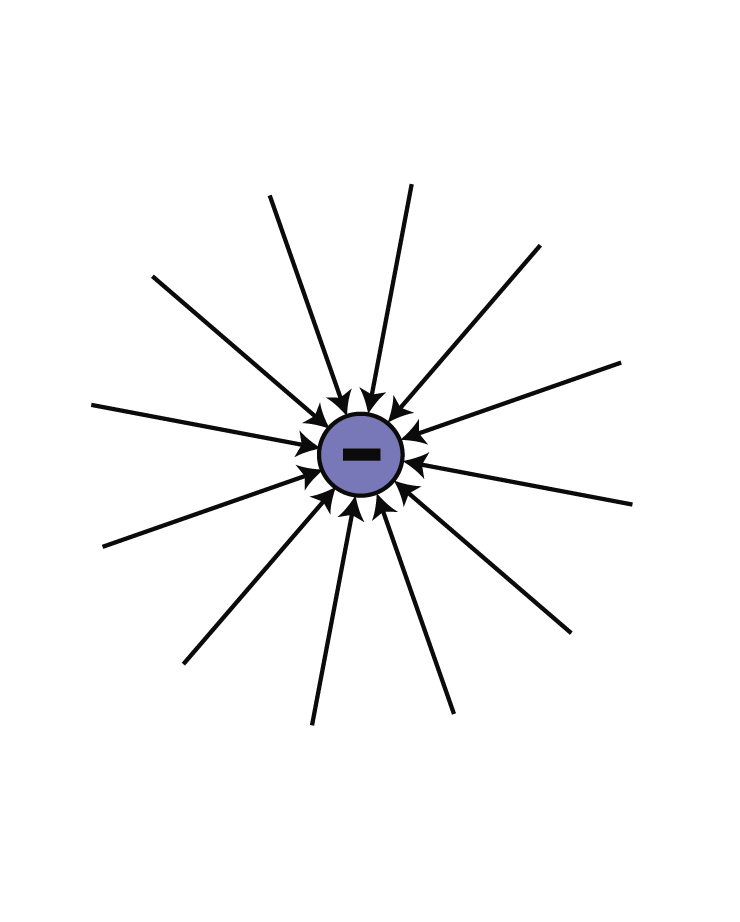
\includegraphics[width=\textwidth]{Images/11.4a}
      \caption{Positive Charge}
      \label{fig:11.4a}
  \end{subfigure}
  \begin{subfigure}[b]{0.3\textwidth}
      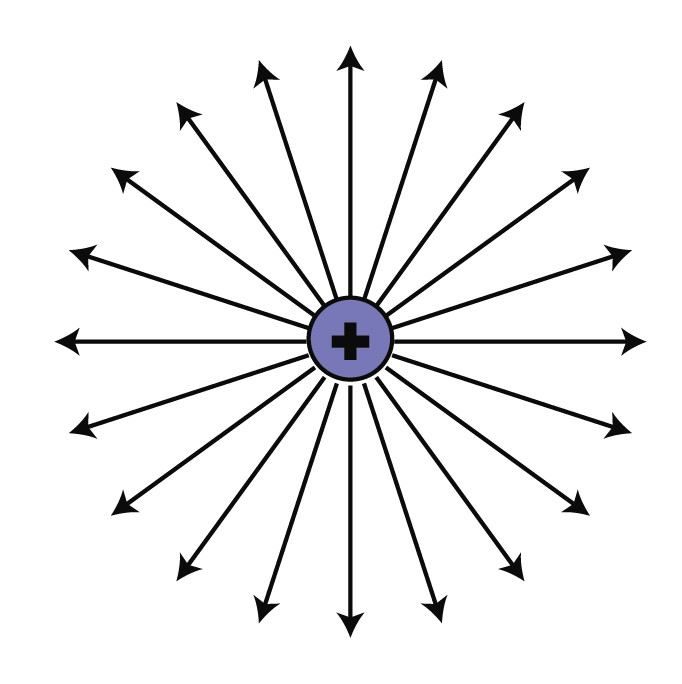
\includegraphics[width=\textwidth]{Images/11.4b}
      \caption{Negative Charge}
      \label{fig:11.4b}
  \end{subfigure}
  \caption[]{Electric field pattern for an isolated positive \& negative charge}
  \label{fig:11.4}
\end{figure}

If medium surrounding the charge ‘q’ is other than vacuum or air,
having dielectric constrant
`$\epsilon_{r}$', then electric intensity will be given by:
\begin{equation}\label{eq:11.16}
  \vec{E} = \frac{1}{4\pi\epsilon_{o}\epsilon_{r}} \frac{q}{r^{2}} \hat{r}
\end{equation}
\subsection{Electric Lines of Force/Electric Field Lines}
\subsubsection{Definition}
\textit{“An electric line of force is a curve so drawn that a tangent to the curve at any point
shows the direction of the field at that point.”}
\subsubsection{Explanation}
Electric lines of force are imaginary lines to show the strength
and direction of a real field. As the strength of the field means
electric field intensity, so electric lines of force represents the
magnitude and direction of electric field. The mapping of electric
field by field lines helps in visualizing the electric field.

The magnitude of the electric field at a certain point is
determined by the density of lines (number of lines per unit area).
The greater the density of lines, the greater will be the magnitude
of electric field. The direction of the field at a given is determined
by drawing a tangent to the field line at that point. Actually,
the field line tells us about the movement of a test charge at
each and every point inside an electric field.
\subsubsection{Properties of Electric Field Lines}
\begin{enumerate}[label=(\roman*)]
\item The density of lines show the direction of electric field.
\item The arrowhead shows the direction of field.
\item The field lines begin from positive charge and terminate on negative
charge, they are continuous in region containing no charge.
\item The lines of force do never cross.If they did cross,
then electric field would have two different directions at
the point of intersection which is not possibe.
Put another way, at the point of intersection,
there would be two tangents possible. As at a given point,
the tangent to the curve represents the direction of field or
the direction in which the test charge will move along at that point,
so the test charge will have to move along two different directions
at the same point and time, which is not possible.
\item The lines of force strike the surface of conductor perpendicularly.
\item The lines of force can not pass through the conductor. As the 
presence of lines implies that there would be an electric field
inside the conductor. As conductor have free charges in them,
so the existence of electric field corresponds the force on those charges,
leading to the flow of charges (electric current),
but no such perpetual currents exist. Hence no electric field exists
inside the conductor body hence no field lines.
\end{enumerate}
\subsubsection{Neutral point/Null point}
\textit{“The point where the net electric field intensity
is zero is called neutral point/null point.”}
It is denoted by ‘N’ (we will discuss its example in next section).
\subsection{Field Lines of Some Electrostatic Charge Distributions}
\subsubsection{For an Isolated Charge}
We have discussed already that field lines for an isolated positive charge are radially outward and radially 
inward for a negative charge extending in space as shown:

\begin{figure}[htbp]
  \centering
  \begin{subfigure}[t]{0.3\textwidth}
      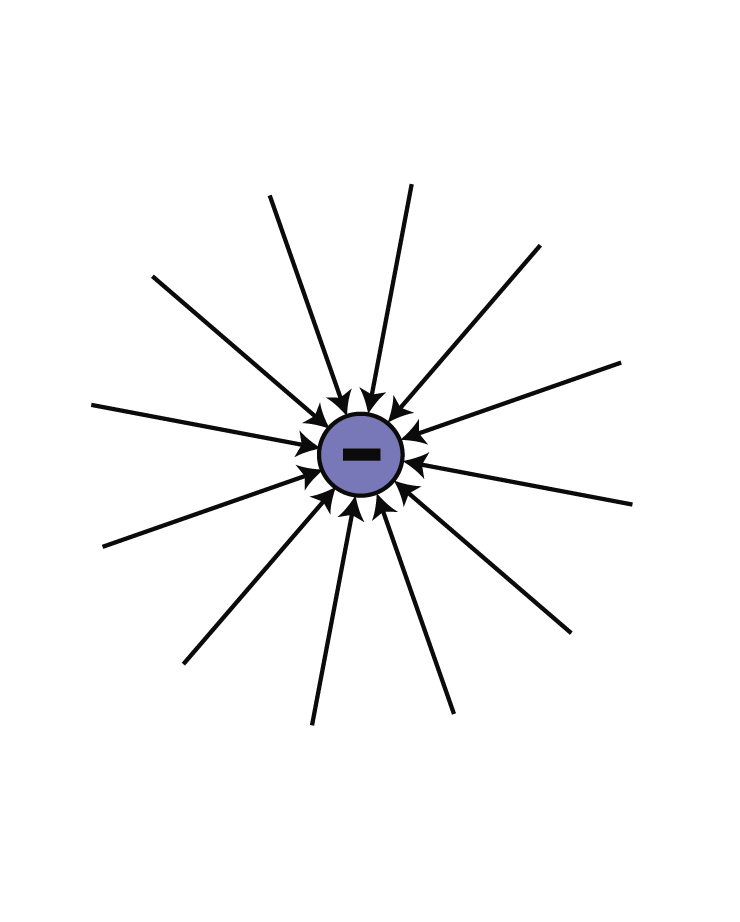
\includegraphics[width=\textwidth]{Images/11.4a}
      \caption{Positive Charge}
      \label{fig:11.5a}
  \end{subfigure}
  \begin{subfigure}[t]{0.3\textwidth}
      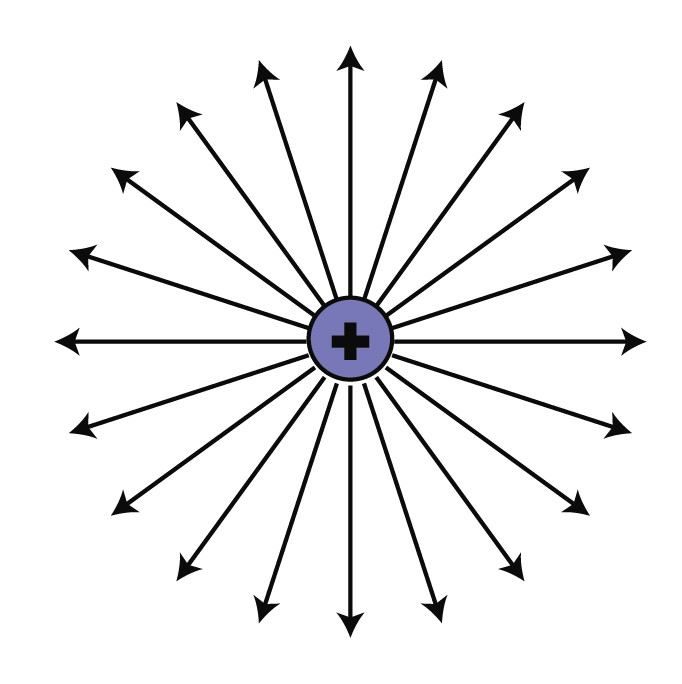
\includegraphics[width=\textwidth]{Images/11.4b}
      \caption{Negative Charge}
      \label{fig:11.5b}
  \end{subfigure}
  \caption[]{Electric field pattern for an isolated positive \& negative charge}
  \label{fig:11.5}
\end{figure}

\subsubsection{For Two Charges of Same Magnitude}
For two charges of same sign and same magnitude (for convenience,
we take them negative), configuration is as shown in \ref{fig:11.6(a)}
The point ‘N’ is neutral point. The number of lines per unit area 
shows the strength of field. So, no lines means no net electric field.
Here, in this case, we assumed both charges of same sign and same magnitude,
hence the point of zero electric field will lie in mid of these chrarges.
For two charges of same magnitudes but opposite signs,
field lines are shown in figure \ref{fig:11.6(b)}.

\begin{figure}[htbp]
  \centering
  \begin{subfigure}[t]{0.3\textwidth}
      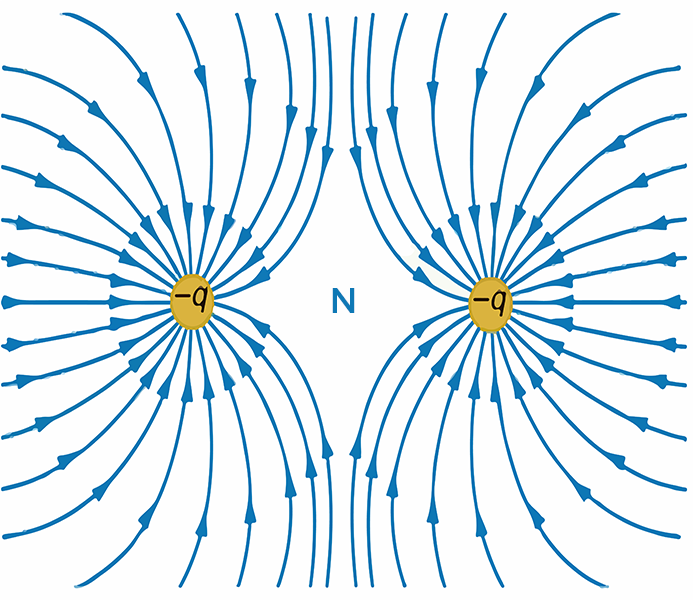
\includegraphics[width=\textwidth]{Images/11.6a}
      \caption{For two negative charges}
      \label{fig:11.6(a)}
  \end{subfigure}
  \begin{subfigure}[t]{0.3\textwidth}
      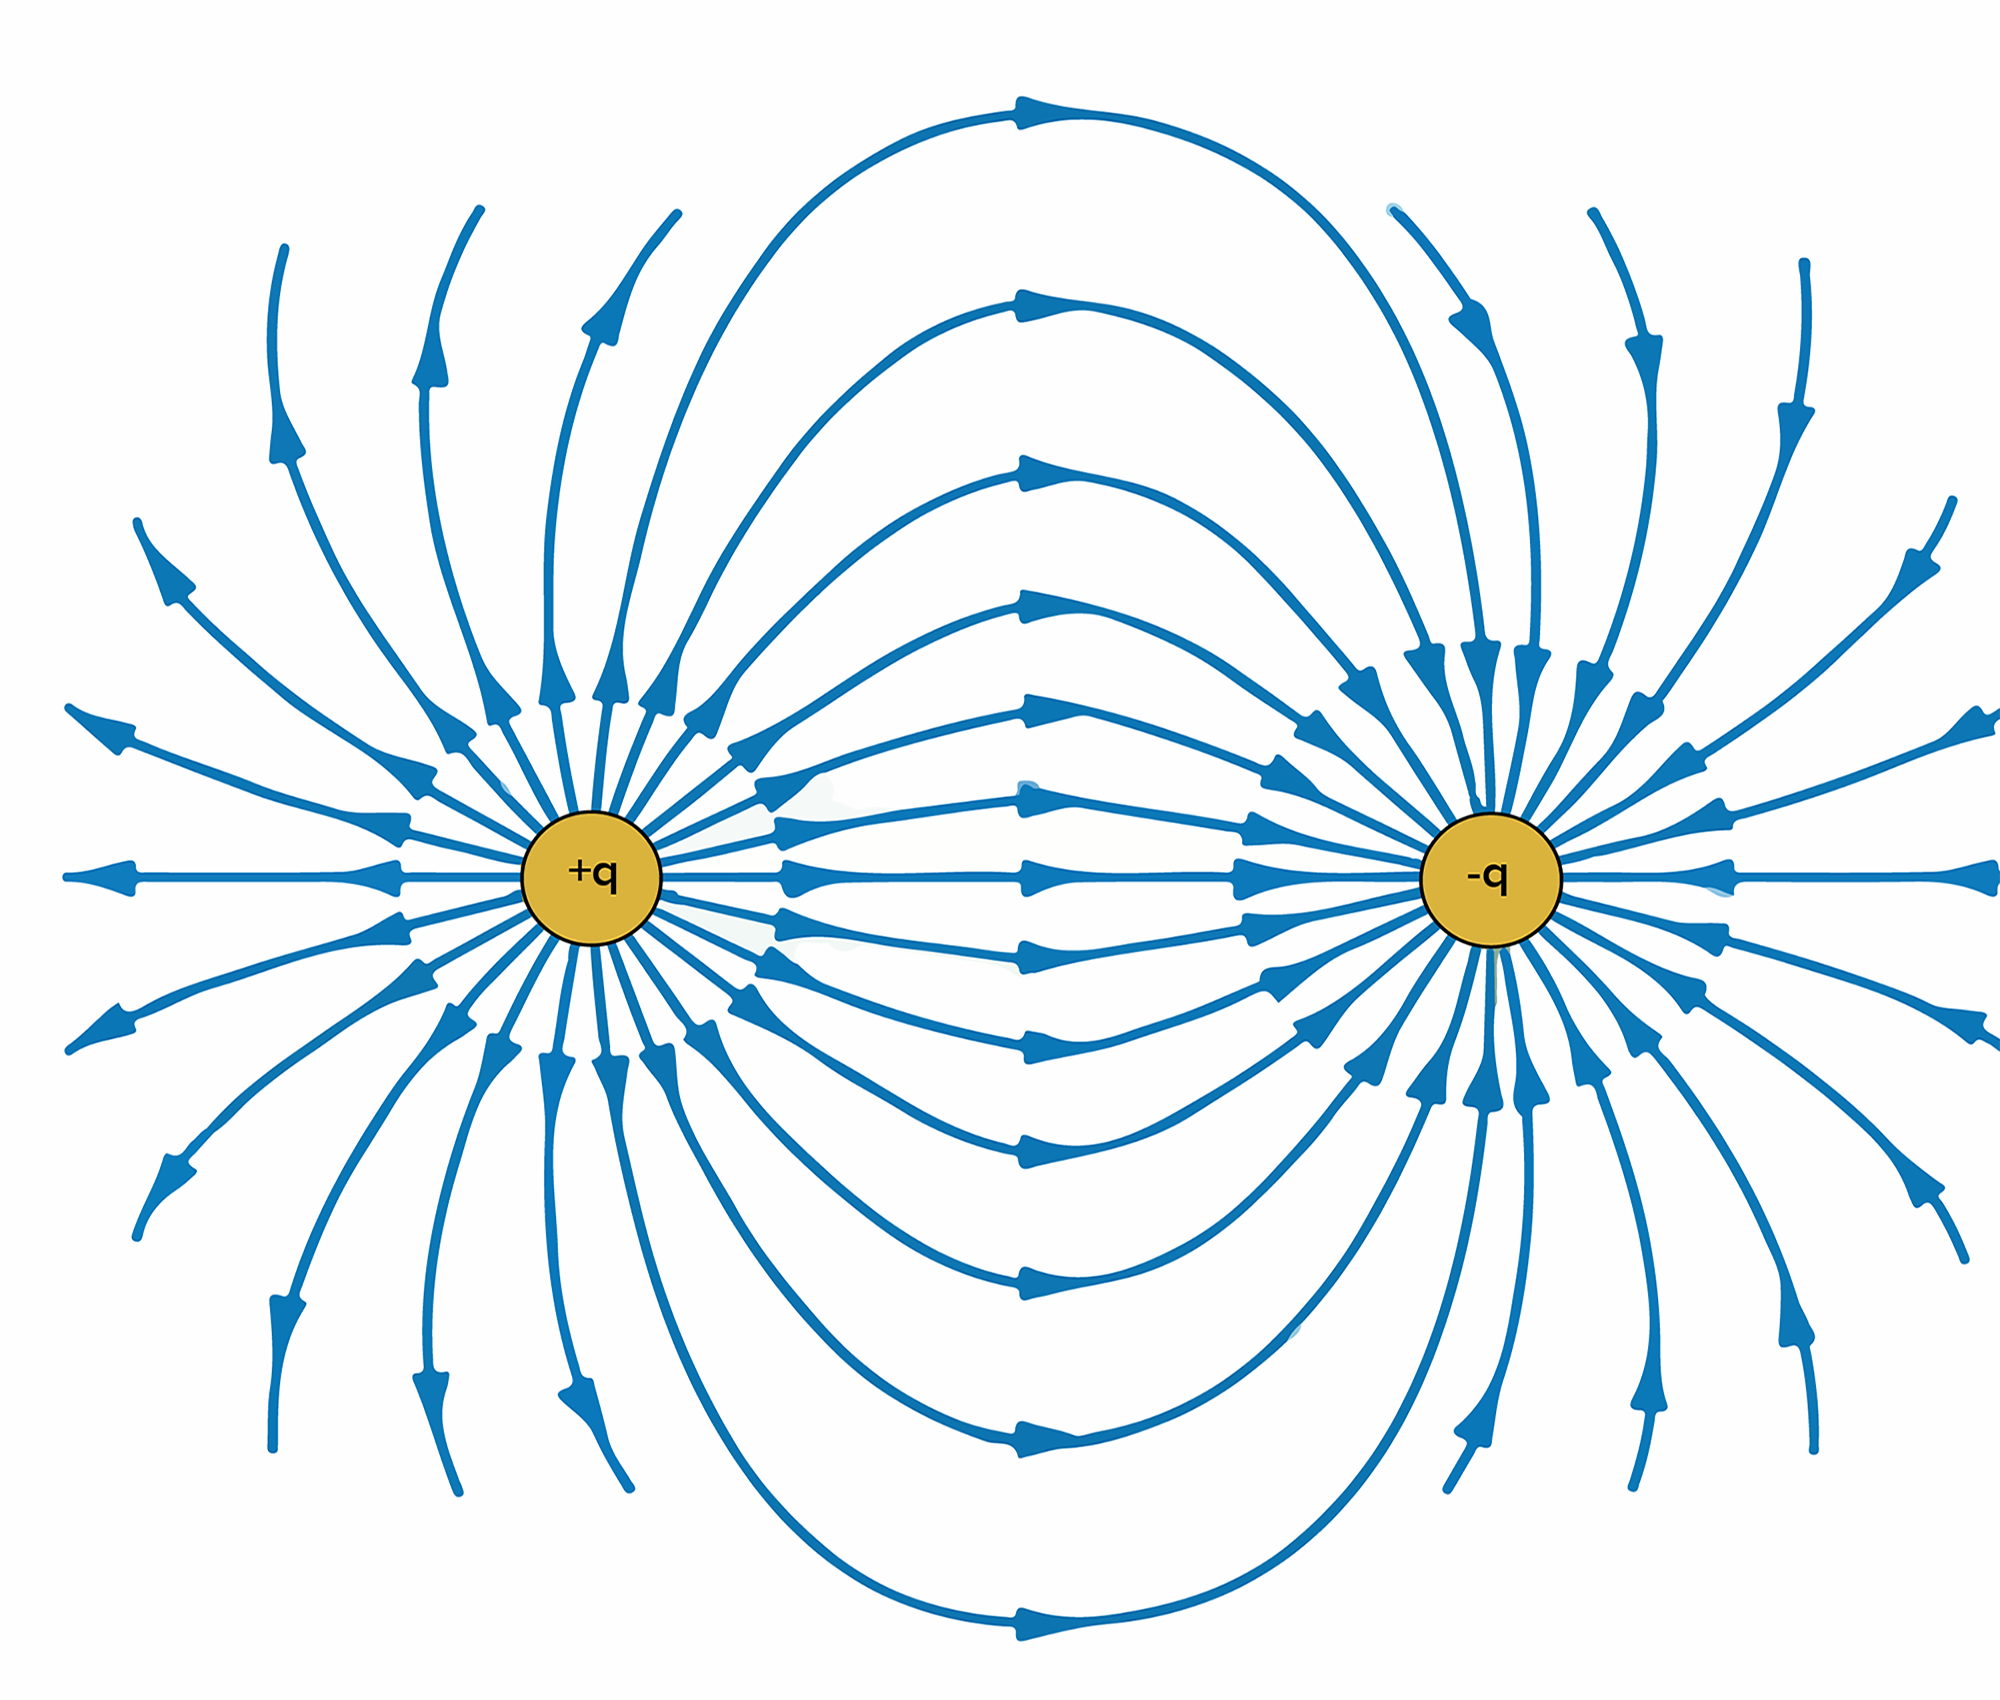
\includegraphics[width=\textwidth]{Images/11.6b}
      \caption{For a positive \& negative charge}
      \label{fig:11.6(b)}
  \end{subfigure}
  \caption[]{Electric field pattern for two charges of same magnitude}
  \label{fig:11.6}
\end{figure}

\subsubsection{Electric Lines Due to a Positive Charge Near a Metal Plate}
Consider an electric charge ‘+q’ placed near a metal plate.
The positive charge will attract the negative charges (electrons) in
the metal plate resulting in the motion of the charges until some
of them reach that surface of the metal which is near the ‘+q’
charge where they will be at rest. Thus the field lines starting from
‘+q’ charge will terminate on the negative charges of the metal plate.
Furthermore,these lines starting from ‘+q’ charge are always perpendicular
to the conductor. The electric lines of force can not pass through the metal.
Electric field is zero inside a conductor under electrostatic conditions.
If it was not so, electric field would exert forces on electrons
causing them to flow establishing current. Since, no such currents do exist,
hence field inside the metal will be zero.
The field configuration of above discussed case is as shown:

\begin{figure}[H]
  \centering
  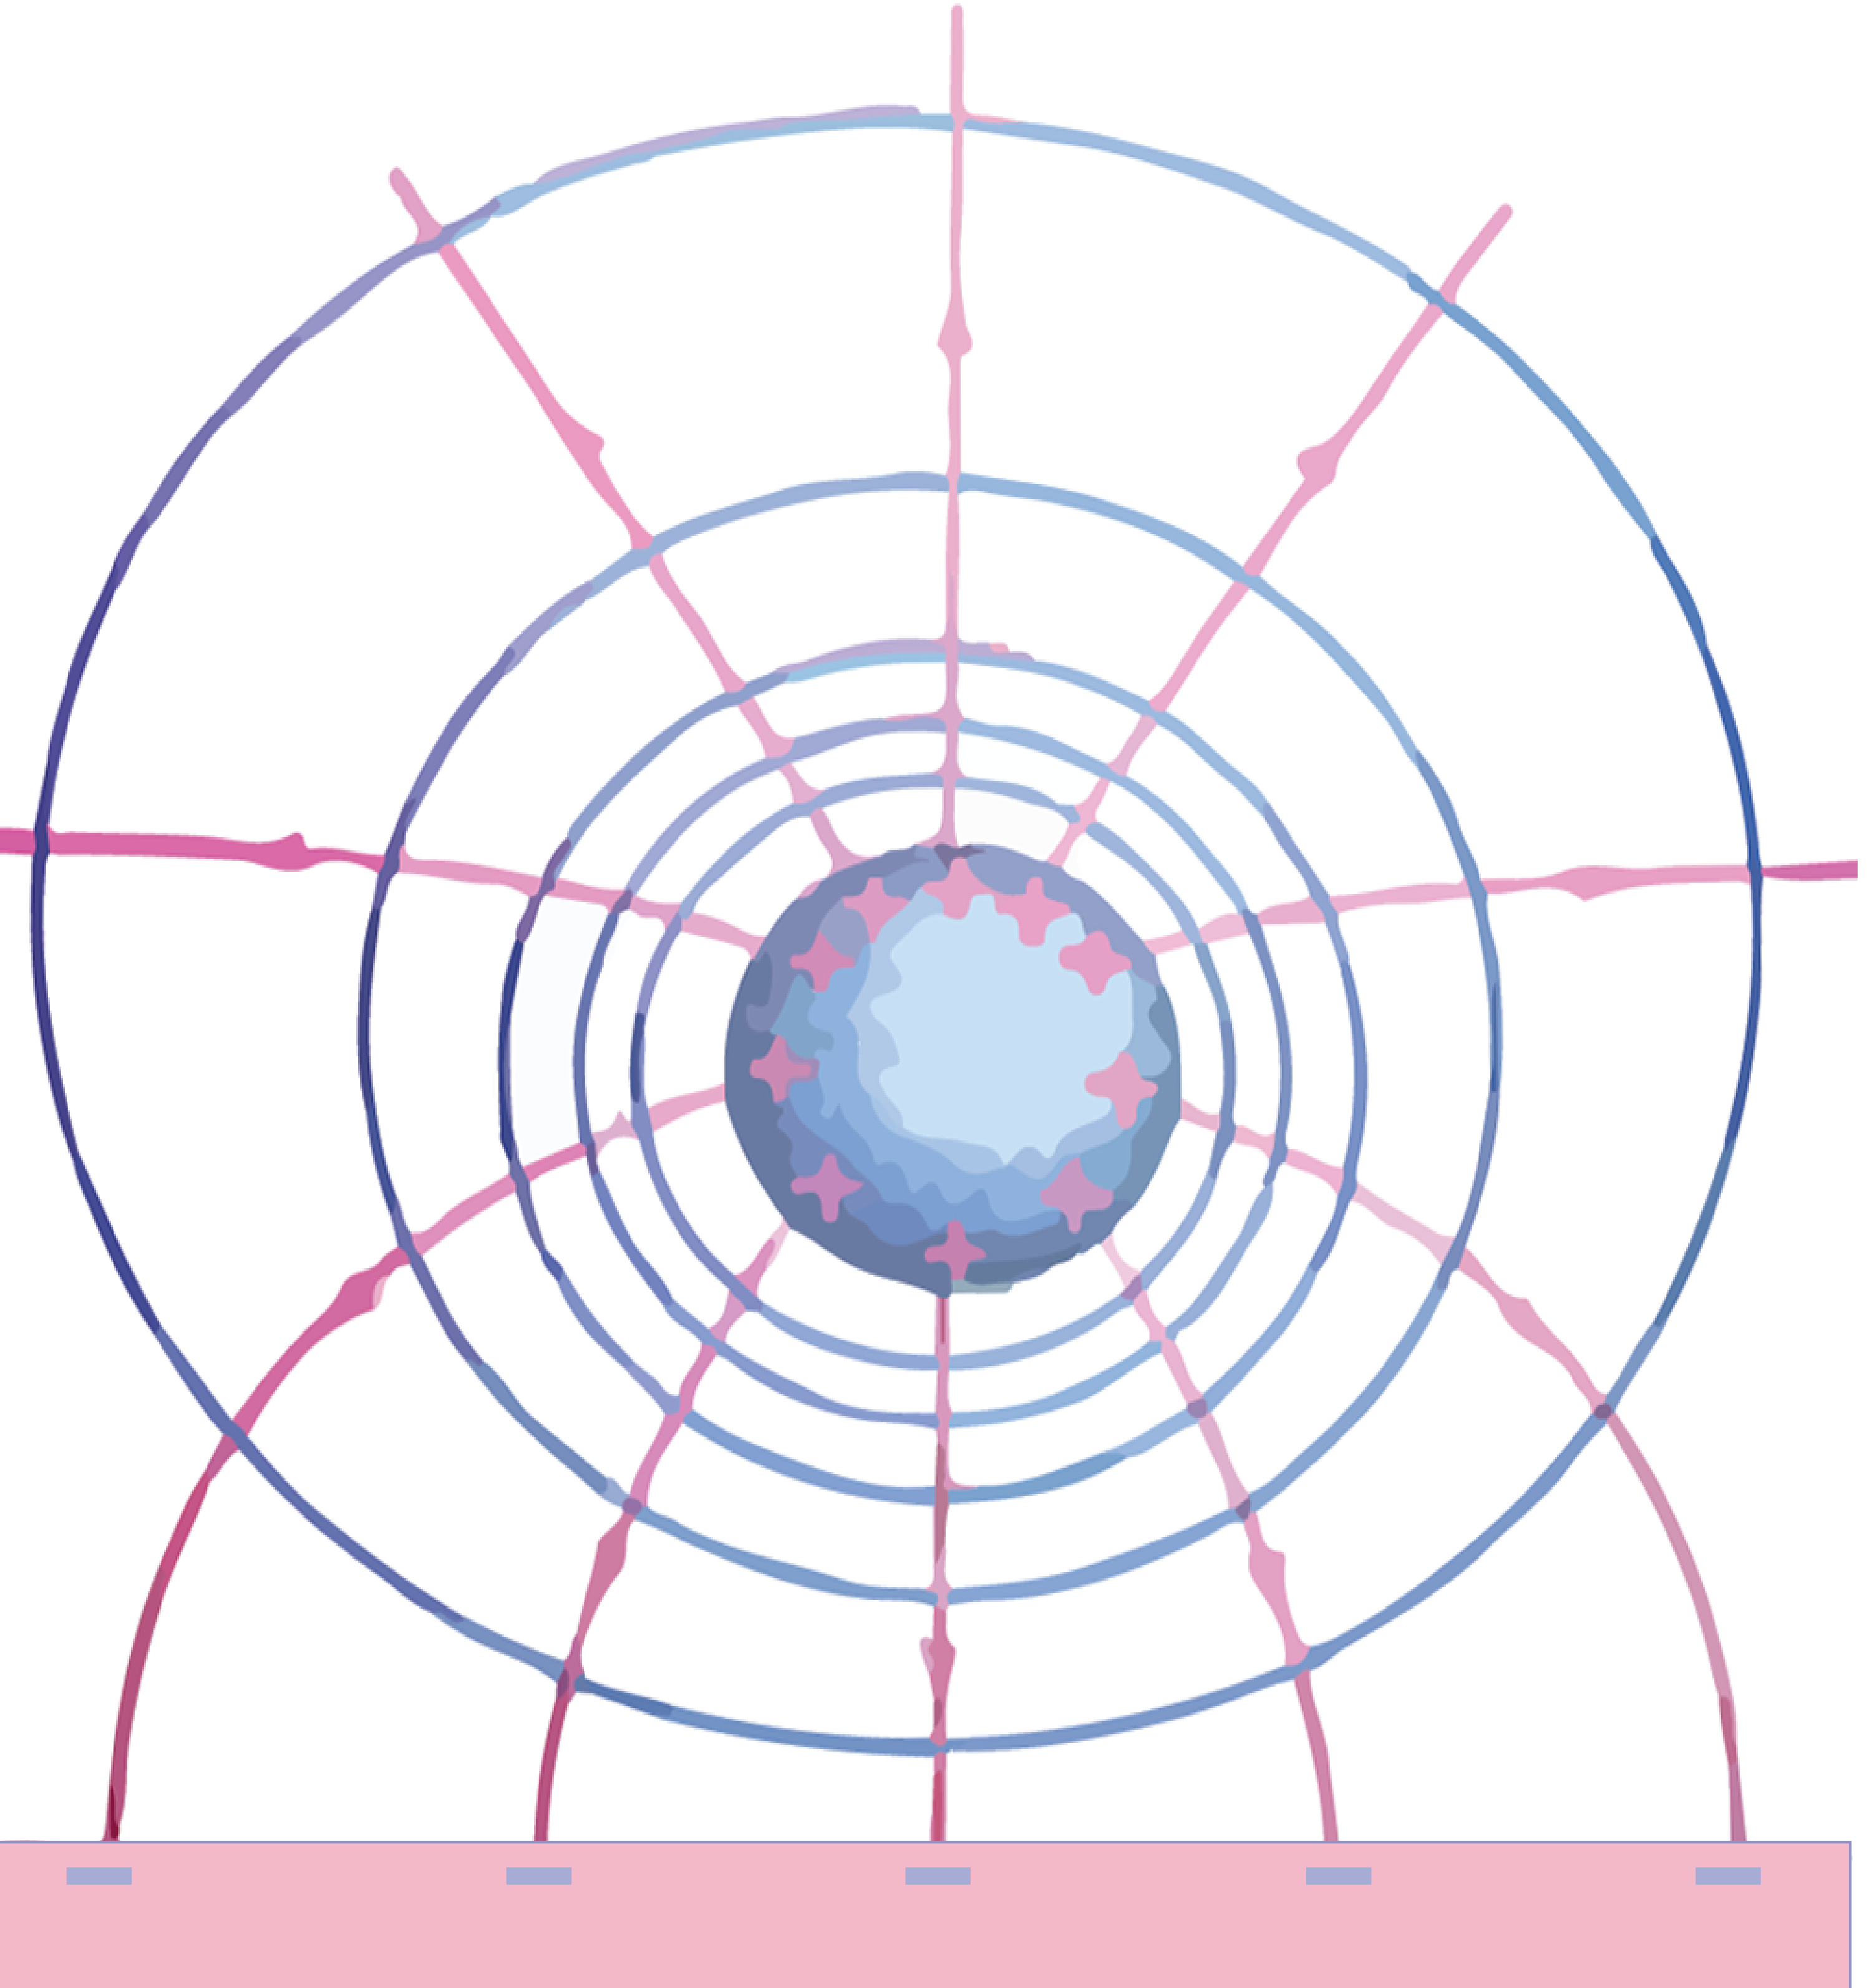
\includegraphics[width=0.4\textwidth]{Images/11.7.png}
  \caption{Field pattern for a positive charge near a metal plate}
  \label{fig:11.7}
\end{figure}

\subsubsection{Uniform Electric Field}
\paragraph{Definition:}
\textit{“A field is said to be uniform in a certain region 
if it has the same magnitude and direction in that region.”}
\paragraph{Explanation:}
From the definition of uniform electric field, it is clear
that the magnitude of field must be constant and direction as well.
As we know that the magnitude of electric field depends upon the number
of lines per unit area,so for uniform electric field, the field lines
are uniformly spaced. The direction the field is is represented by the
arrows, hence for same direction,
they(lines) must point in the same direction.
\paragraph{Production of Uniform Electric Field:}
A uniform electric field can be produced by connecting the
terminals of a baatery connected to two large parallel metal plates.
If the plates are of finite length,then the lines of force are bulging
at the ends of the plates. This non-uniform field at the edges
of the plates is called ‘fringing field’. In order to avoid fringing field,
the paltes must be of infinite length. Practically, plates are said to
be of infinite length when the distance between them is much smaller than
their dimensions. The field pattern is as shown:

\begin{figure}[H]
  \centering
  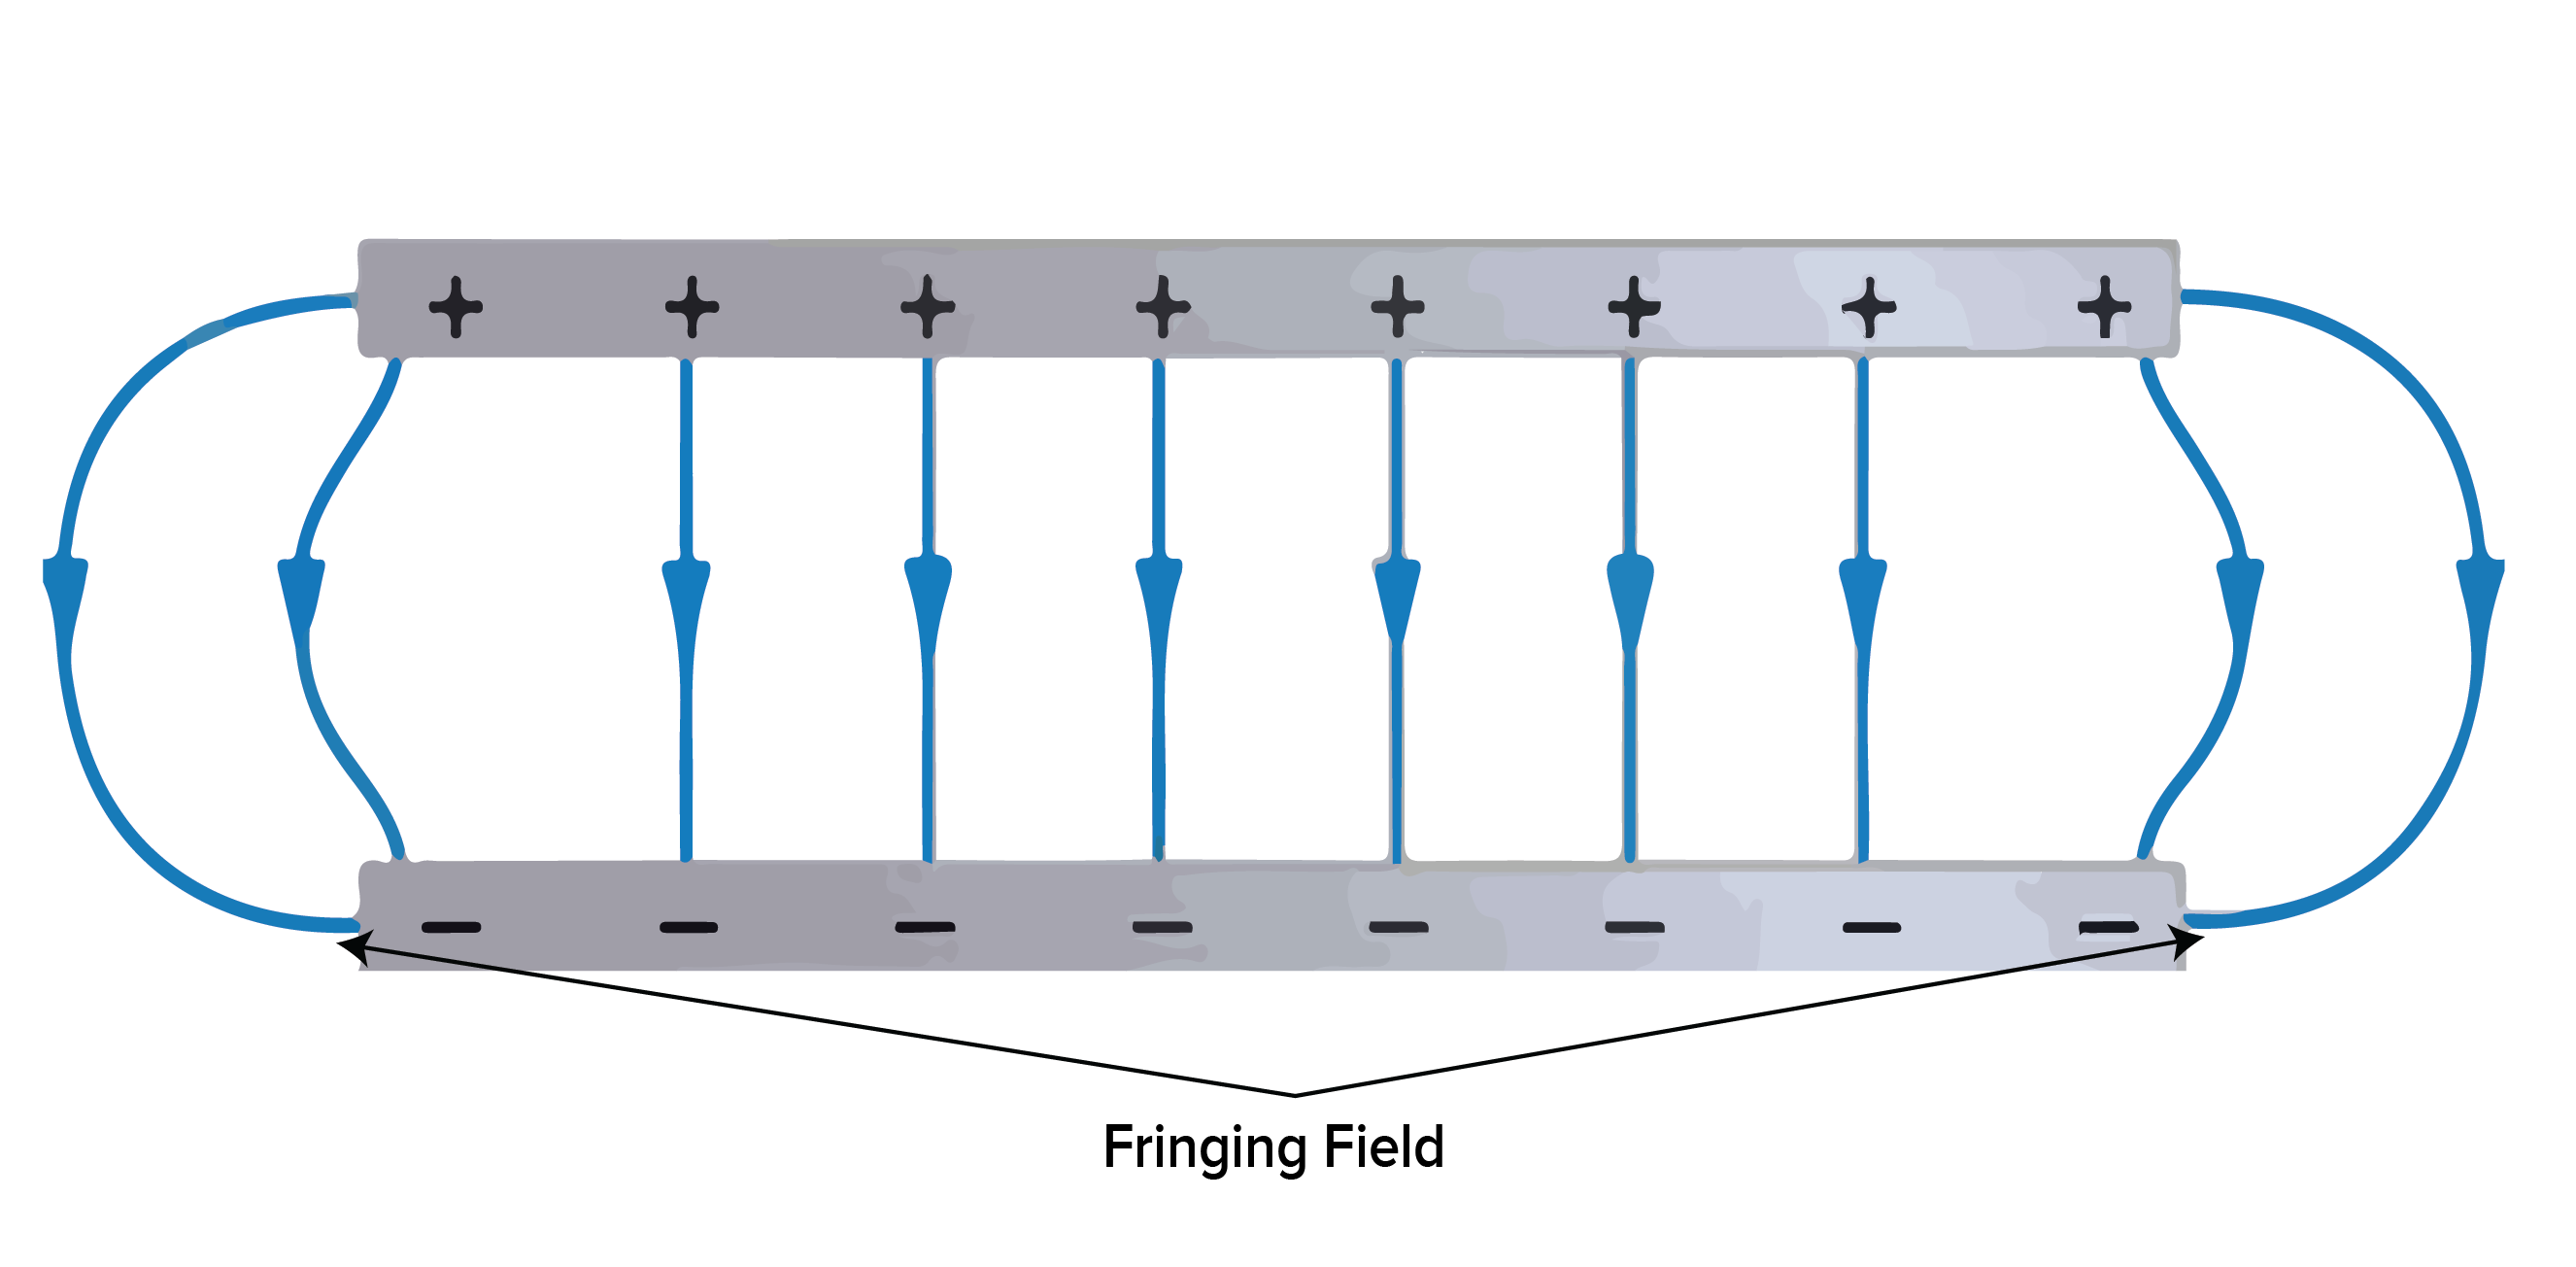
\includegraphics[width=0.6\textwidth]{Images/11.8.png}
  \caption{Uniform Electric Field with a `fringing field'}
  \label{fig:11.8}
\end{figure}

\section{Electric Flux}
\textit{“The number of electric lines passing through the area placed in the electric field,is called electric flux.”}
\subsection*{Symbol}
It is denoted by $\Phi_{E}$ (Greek alphabet phi) where the subscript ‘E’ is for electric.
\subsection*{Explanation}
In the above definition,we have discussed two vector quantities,
electric field lines mean electric field intensity. The magnitude of
electric field intensity is, \textit{“the number of lines per unit area
placed perpendicular to E.”} The second vector involved in the
definition of electric flux is Area. The magnitude of the area vector
is equal to the area of the plane occupied and direction is always normal
to the surface/plane shown by `$\hat{A}$' or `$\hat{n}$'.
Here we considered a flat circular surface, area vector is shown,
the direction is shown by normal unit vector `$\hat{n}$'.
\subsection*{Mathematical Form}
If $\vec{E}$ is the electric field intensity which is uniform over a certain area,
then the electric flux will be given by:
\begin{equation}\label{eq:11.17}
  \Phi_{E}  = \vec{E}.\vec{A}
\end{equation}
Hence, it is the dot product of previously dicussed two vector
quantities $\vec{E}$ and $\vec{A}$.
Using usual notations we can write it as:
\begin{equation}
  \Phi_{E} = EAcos\phi
\end{equation}
where $Acos\phi$ is the component of area held perpendicular to
E (But its direction will be along E).
This equation is the mathematical form of flux at any angle.
In the figure, the area component which is perpendicular
to field lines is  `$A_{\bot}$'. Note that only this component contributes
to electric flux, the lines of forces just skim through `$A_{\parallel}$'.
Resolving area vector into its $\hat{i}$ and $\hat{j}$ components,
the component which is along the direction of electric field is $Acos\phi\:\hat{i}$
which is actually the vector associated with the same area component
that is held perpendicular to electric field lines and contributing
to flux (As its direction is perpendicular to `$A_{\parallel}$').
So we defined electric flux as the product of electric
intensity and the component of area vector along the direction of $\vec{E}$.

\subsection*{Maximum Flux}
If the surface is placed perpendicular to electric field such
that surface area vector is parallel to the direction of electric field E,
then maximum number of lines of force will pass through the surface.
Consequently, maximum electric flux will pass through the surface.
(Note that $\phi$ is the smaller angle between $\vec{E}$ and area vector
$\vec{A}$ which is perpendicular to the plane of area).
This is shown in figure \ref{fig...}:
Using flux definition:
\begin{equation}
  \Phi_{E} = EAcos\phi \nonumber
\end{equation}
Here $\phi = 0^{\circ}$, So,
\begin{equation}
  \Phi_{E} = EAcos(0^{\circ}) \nonumber
\end{equation}
\begin{equation}
  \Phi_{E} = EA \nonumber
\end{equation}
This can be physically understood by another way.
Since `$A_{\bot}$' is the only area component contributing to flux and there
is no parallel component of area `$A_{\bot}$. So,only the vector area related with `...'
will be involved in defining flux i.e. $Acos\:\phi$, which is equal to the
whole area vector, and writing in magnitude form we have flux equal to $EA$.

\subsection*{Zero Flux}
If the surface is placed parallel to the electric field lines such that
area vector $\vec{A}$ is normal to the electric field $\vec{E}$,
then the maximum number of lines will pass through the surface. Consequently,
no electric flux will pass through the surface, as shown:
Mathematically,
\begin{equation}
  \Phi_{E} = EAcos\phi \nonumber
\end{equation}
Here $\phi = 90^{\circ}$, So,
\begin{equation}
  \Phi_{E} = EAcos(90^{\circ}) \nonumber
\end{equation}
\begin{equation}
  \Phi_{E} = 0 \nonumber
\end{equation}

\noindent\textbf{Note:} We defined `$A_{\bot}$ and `$A_{\parallel}$' be the components of the surface on the basis of
their orientation relative to field lines.

\subsection*{Nature}
Since,electric flux is the dot product of $\vec{A}$ and $\vec{A}$, so it is a scalar quantity.

\subsection*{Units}
The S.I unit of electric flux is $Nm^{2}C^{-1}$.
\subsection{Flux Through an Arbitary Shaped Body}
We defined flux to be equal to $\vec{E}.\vec{A}$ which is applicable
only if `E' is uniform over the whole area A, i.e. for flat surfaces.
If the surface is not flat, then equation $\vec{E}.\vec{A}$ can not be
applied directly, because the angle between E and A changes from place
to place.In such cases, the product $\vec{E}.\vec{A}$ defines flux only
for small area piece which is considered flat. Therefore, to find flux for
an uneven surface (open or closed), we divide the surface into small flat
pieces $\Delta A_{1},\:\Delta A_{2},\:\Delta A_{3},...,\:\Delta A_{n}$.
as shown:



The area vectors of these area components are $\vec{\Delta A_{1}},\:\vec{\Delta A_{2}},\:\vec{\Delta A_{3}},...,\:\vec{\Delta A_{n}}$.
The electric field intensity at these area pieces are $\vec{E_{1}},\:\vec{E_{2}},\:\vec{E_{3}},...,\:\vec{E_{n}}$ repectively.
The small amount of flux `$\Delta \Phi_{1}$' through `$\Delta A_{1}$' is defined as:
\begin{equation}
  \Delta \Phi_{1} = \vec{E_{1}}.\Delta \vec{A_{1}} \nonumber
\end{equation}
Similarly,
\begin{equation}
  \Delta \Phi_{2} = \vec{E_{2}}.\Delta \vec{A_{2}} \nonumber
\end{equation}
Hence for n\textsuperscript{th} patch, 
\begin{equation}
  \Delta \Phi_{n} = \vec{E_{n}}.\Delta \vec{A_{n}} \nonumber
\end{equation}
So, the total flux through the surface will be:
\begin{equation}
  \Phi_{T} =  \Phi_{1}+ \Phi_{2}+ \Phi_{3}+...+ \Phi_{n} \nonumber
\end{equation}
Putting respective values:
\begin{equation}
  \Phi_{T} = \vec{E_{1}}.\Delta \vec{A_{1}}+\vec{E_{2}}.\Delta \vec{A_{2}} +\vec{E_{3}}.\Delta \vec{A_{3}}+...+\vec{E_{n}}.\Delta \vec{A_{n}} \nonumber
\end{equation}
Which in compressed notation:
\begin{equation} \label{eq:11.19}
  \Phi_{T} = \sum_{i=1}^{n} \vec{E_{i}}.\Delta \vec{A_{i}} 
\end{equation}
\subsection{Flux through a closed Arbitrary Surface}
Let us consider a closed sufrace of arbitrary with the positive normal
taken outward from the volume beig closed.In case of closed surface,
the electric flux may be positive, negative or zero depending upon
the number of lines entering or leaving the surface.We discuss it as:

\begin{enumerate}[label=(\roman*)]
\item The electric flux is positive,if net number of lines are leaving the surface.Since positive charge is a source of field lines,so it means that there is a source of libes inside the surface,i.e.positive charge.
Mathematically,for closed surace of abitrary shape:
\begin{equation} 
  \Phi_{T} = \sum_{i=1}^{n} \vec{E_{i}}.\Delta \vec{A_{i}} \nonumber
\end{equation}
And this implies that there is a source of field lines inside the surface.
The number of lines leaving the surface are more than number of lines entering,flux would be negative for lines entering and it would be positive for lines leaving and hence net flux would be positive.
\item The electric flux through a closed surface will be negative,
if net number of lines are entering the surface or more field lines are entering than leaving the surface;there is a sink of field lines in the closed surface i.e. a negative charge as field lines terminate on negative charge.
\item The electric flux will be zero if number of lines entering is 
equal to the number of lines leaving the surface or no field lines
intercpepting the surface. This is possible when there is no net charge
because net charge is a source or sink of lines.
\end{enumerate}
\section{Gauss’s Law}
\subsection*{Background}
The electric field of a given charge distribution can be calculated
using Coloumb’s law. But sometimes field calculation using Coulomb’s law
becomes very difficult. An alternative method to calculate the electric
field of a given charge distribution relies on theorem called ‘Gauss’s law’
given by Karl Friedrich Gauss\footnote{German mathematician and astronomer (1777-1855) Gauss received a doctoral degree
in Mathematics from the University of Helmsted in 1799. In addition to his
work in electromagnetism, he made contributions in mathematics,
number thoery, statistics and mecahnics.}.
It provides a realtionship between the net electric flux
through the closed surface and the net charge enclosed by that surface.
\subsection*{Statement}
\textbf{\textit{“The net electric flux through any closed surface is equal to $\frac{1}{\epsilon_{o}}$
times the charge ‘q’ enclosed by that surface.”}}
\subsection*{Explanation}
Gauss’s law provides a simple relationship between the electric flux
through any closed surface and the total charge inside that surface.
The charges inside the surface can
be either a single point charge or a number of charges.

In order to derive an expression for Gauss’s law,
let us consider a closed surface (for convenince we take a sphere)
of radius `r' having a point charge ‘q’
at its centre as shown in figure \ref{fig...}.
As the direction of electric field intensity E varies from place to place,
so in order to calculate electric flux, we divide the whole surface into ‘n’
number of small pieces having area $\Delta A_{1},\:\Delta A_{2},\:\Delta A_{3},...,\:\Delta A_{n}$.
Here,we considered a sphere,so two things are important:
\begin{enumerate}[label=(\roman*)]
  \item Electric field intensity is same at every point as they are equidistant from the charge.
  \item As field is radial, it means that at every point E and A are in same direction i.e. the angle between E and A at every point will be zero degree.
\end{enumerate}
Now, we know that the total flux through area $\Delta A_{1}$ will be:
\begin{equation}
  \Delta \Phi_{1} = \vec{E_{1}}.\Delta \vec{A_{1}} \nonumber
\end{equation}
Similarly,
\begin{equation}
  \Delta \Phi_{2} = \vec{E_{2}}.\Delta \vec{A_{2}} \nonumber
\end{equation}
Hence for n\textsuperscript{th} patch, 
\begin{equation}
  \Delta \Phi_{n} = \vec{E_{n}}.\Delta \vec{A_{n}} \nonumber
\end{equation}
Since,
\begin{equation}
  E_{1} = E_{2} = E_{3} = E_{n} = E \nonumber
\end{equation}
And the total flux will be:
\begin{equation}
  \Phi =  \Phi_{1}+ \Phi_{2}+ \Phi_{3}+...+ \Phi_{n} \nonumber
\end{equation}
Putting respective values:
\begin{equation}
  \Phi = \vec{E}.\Delta \vec{A_{1}}+\vec{E}.\Delta \vec{A_{2}} +\vec{E}.\Delta \vec{A_{3}}+...+\vec{E}.\Delta \vec{A_{n}} \nonumber
\end{equation}
Since, field is radial, hence:
\begin{equation}
  \Phi = E\Delta A_{1} + E\Delta A_{2} + E\Delta A_{3+...+E\Delta A_{n}} \nonumber
\end{equation}
\begin{equation}
  \Phi = E(\Delta A_{1} + \Delta A_{2} + \Delta A_{3+...+\Delta A_{n}}) \nonumber
\end{equation}
\begin{equation}\label{eq:11.20}
  \Phi = E\sum_{surface} \Delta A 
\end{equation}
Since, electric field at a distance ‘r’ due to charge ‘q’ will be:
\begin{equation}
  E = \frac{q}{4\pi\epsilon_{o}r^{2}} \nonumber
\end{equation}
Also we know that in case of sphere:
\begin{equation}
  \sum_{surface} \Delta A = 4\pi r^{2} \nonumber
\end{equation}
Putting these values in equation \ref{eq:11.20}
\begin{equation}
  \Phi = \frac{q}{4\pi\epsilon_{o}r^{2}} 4\pi r^{2} \nonumber
\end{equation}
\begin{equation}\label{eq:11.21}
  \Phi = \frac{q}{\epsilon_{o}}
\end{equation}
Equation \ref{eq:11.21} defines Gauss’s law for point charge. It is clear that electric flux is independent of:
\begin{enumerate}[label=(\roman*)] 
\item The shape of closed surface.
\item The radius(size) of the closed surface.It means that if radius
is made very small or large, still $\frac{q}{\epsilon_{o}}$ lines will come from ‘q’.
\end{enumerate}
And equation also tells that the flux depends upon:
\begin{enumerate}[label=(\roman*)]
\item The amount of charge enclosed.
\item The medium surrounding the charge.
\end{enumerate}
\subsection*{Conclusion}
We conclude that each positive charge must have $\frac{q}{\epsilon_{o}}$ lines coming from it.
A negative charge will have the same number of lines going through it.
Another important thing is that whatever the shape of the closed surface
is flux will be same for a given charge placed inside the surface in a
medium. We assumed the closed surface as sphere which helped in making
our calculation easy. At last we found that it does not matter that
what is the shape of surface, it should be just closed and must enclose
a charge to give out flux.
\subsection{Electric Flux due to Many Charges}
To formulate Gauss’s law for many charges,
let us consider point charges q\textsubscript{1}, q\textsubscript{2},
q\textsubscript{3},..., q\textsubscript{n}
inside a closed surface S, of some arbitrary shape, as shown:
We know that all the flux lines coming from q\textsubscript{1}’ passes through the surface ‘S’,
therefore from Gauss’s law, flux due to ‘q\textsubscript{1}’ will be:
\begin{equation}
  \Phi_{1} = \frac{q_{1}}{\epsilon_{o}} \nonumber
\end{equation}
Similarly,
\begin{equation}
  \Phi_{2} = \frac{q_{2}}{\epsilon_{o}} \nonumber
\end{equation}
And,
\begin{equation}
  \Phi_{3} = \frac{q_{3}}{\epsilon_{o}} \nonumber
\end{equation}
Hence due to n\textsuperscript{th} charge:
\begin{equation}
  \Phi_{n} = \frac{q_{n}}{\epsilon_{o}} \nonumber
\end{equation}
As total flux is given by:
\begin{equation}
  \Phi =  \Phi_{1}+ \Phi_{2}+ \Phi_{3}+...+ \Phi_{n} \nonumber
\end{equation}
Putting respective values:
\begin{equation}
  \Phi = \frac{1}{\epsilon}\times (q_{1}+q_{2}+q_{3}+...+q_{n}) \nonumber
\end{equation}
Since,
\begin{equation}
  q_{1}+q_{2}+q_{3}+...+q_{n}) = Q \nonumber
\end{equation}
So, we get:
\begin{equation}\label{eq:11.22}
  \Phi = \frac{Q}{\epsilon_{o}}
\end{equation}
Note that ‘Q’ is the net charge which is the algebraic
sum of all the charges. It is also important to note that the
electric field due to a charge outside the surface contributes zero
electric flux through the surface because as many field lines
due to that charge enter as leave it.In section before Gauss’s law,
we discussed positive, negative and zero electric flux through an
arbitrary closed surface by using definition of electric flux.
Now, we can relate the same using Gauss’s law. We can further specify equation
\ref{eq:11.22} by writing it as:
\begin{equation}\label{eq:11.23}
  \Phi = \frac{Q_{enclosed}}{\epsilon_{o}}
\end{equation}
Now we discuss three cases:
\begin{enumerate}[label=(\roman*)] 
\item The algebraic sum of ‘+q’ and ‘-q’ charges,
if equal to zero i.e. $Q = 0$,then net flux using above equation 
will be zero. In other case, if there is no charge enclosed, then flux
 will again be zero.
\item If there is a positive charge or sum of charges taking into account
their signs comes out to be positive, then electric flux would be positive.
More number of lines will be leaving thean the number of lines entering.
\item If the closed surface has a negative charge or a net negative charge,
the flux will be negative. The flux will be inward flux, i.e. more lines
will be enteing than the leaving lines provided the normal is taken outward.
\end{enumerate}

\subsection{Applications of Gauss’s Law}
Gauss’s law provides a convenient method to calculate electric field in case of sufficiently symmetric charge distribution.
Here we discuss some applications of Gauss’s law:

\subsubsection{Absence of Electric Field and Charge Inside
a Condctor and Location of Excess Charge on a Conductor}
Under steady state conditions, electric field is zero inside a
metal or conductor. This statement is proved by following considerations;
Conductors have charges in them, which are free to move.
If a resultant field E exists inside the conductor,
these charges will experience a force due to the field.
They will move and internal currents will set-up. Eventually,
within fractions of second, electrostatic equilibrium is achieved.
The internal currents will stop. When no electric current flows,
resultant force on the charges (electrons) in the conductor must be zero.
Since, electric field is responsible for exerting force on the charges,
hence, when electrostatic equilibrium is achieved, the electric field in
the interior of conductor must be zero.
In fact, Gauss’s law can be used to show that an excess charge
placed on an insulated conductor, resides on its outer surface.
For this purpose, consider an isolated conductor carrying an excess charge
‘q’. Take Gaussian surface ‘S’ shown by dotted line. ‘S’ lies inside just
below the actual suface of the conductor as shown:

%figure
As under steady state conditions,
the electric field inside a conductor is zero. Applying Gauss’s law to
the Gaussian’s surface ‘S’, 
we have:
\begin{equation}\label{eq:11.24}
 \sum_{surface} \vec{E}.\vec{\Delta A}  = \frac{Q}{\epsilon_{o}}
\end{equation}
As ‘E’ is zero.so $\sum_{surface} \vec{E}.\vec{\Delta A} = 0$. Now, $\epsilon_{o} \neq \infty$,
as it has a finite value equal to $8.85\times10^{-12}\:C^{2}/Nm^{2}$,
so above equation implies:
\begin{center}
  $Q=0$
\end{center}
This means that there is no charge inside the Gaussian’s surface `S'.
As this surface lies just below the actual surface of the conductor,
having no charge inside it.
This means that the charge is on the actual surface of the conductor.

\subsubsection{Electric Field Intensity due to a Charged Conducting Spherical Shell}
\paragraph{Shell:}\textbf{\textit{“Any hollow enclosure with a covering is called a shell.”}}
\paragraph{Calculation of Electric Field:}
We are interested in the calculation of electric field due to a
charged conducting sphericall shell. For this purpose,
consider a metallic shell of radius ‘R’ having a positive charge ‘Q’.
We know that the charge will distribute itself uniformly on the
conducting surface. As shell has an interior and exterior,
therefore, we will find electric intensity seperately for
interior and exterior of charged conducting spherical shell.
\paragraph{Field at the Interior:}
Suppose we want to find the intensity of the field at an interior
point ‘B’ at a distance $r_{B} < R$ from the centre of the shell.
Through the point ‘B’ construct a ‘Gaussian’s surface’ (Sphere)
of radius ‘$r$’ with centre at the centre of the shell, as shown:

%Figure

Since there is no charge inside the gaussian surface,
hence Gauss’s law gives:

\begin{equation}
  \sum_{surface} \vec{E_{B}}.\vec{\Delta A}  = \frac{Q}{\epsilon_{o}} = 0 \nonumber
\end{equation}
The charge distribution is spherically symmetric. This implies that $\vec{E_{B}}$
is radial and has a constant magnitude $E_{B}$ at all points on the
gaussian’s surface at the radial distance ‘$r_{B}$’ from the centre of
the shell. The vector $\vec{\Delta A}$ at every point is also radial,
So we can write above equation as:
\begin{equation}
  E_{B}\sum_{surface} \Delta A = 0 \nonumber
\end{equation}
As $\sum_{surface} \Delta A \neq 0$ and equal to $4\pi r^{2}$, So
\begin{equation}
  E_{B}(4\pi r^{2}) = 0 \nonumber
\end{equation}
Hence,
\begin{equation}
  E_{B} = 0 \nonumber
\end{equation}
As ‘B’ was chosen as an arbitrary point, therefore, we conclude
that the field inside a charged conducting spherical shell is zero.
\paragraph{Field at the Exterior:}
Let us how find the field at an arbitrary point P,
which is outside the shell and at a ditance `$r_{p}$' from the
centre of the shell. Through P, construct a gaussian surface of 
radius `$r_{p}$' concentric with the shell, as shown:
Applying Gauss’s law:
\begin{equation}
  \sum_{surface} \vec{E_{P}}.\vec{\Delta A}  = \frac{Q}{\epsilon_{o}} \nonumber
\end{equation}
Because of spherical symmetry, $E_{p}$ must be radial. $\vec{\Delta A}$
is also radial. So, above equation implies:
\begin{equation}
  E_{P}\sum_{surface} \Delta A = \frac{Q}{\epsilon_{o}} \nonumber
\end{equation}
As $\sum_{surface} \Delta A = 4\pi r^{2}$, So
\begin{equation}
  E_{P}(4\pi r^{2}) = \frac{Q}{\epsilon_{o}}  \nonumber
\end{equation}
\begin{equation}\label{eq:11.25}
  E_{P} = \frac{Q}{4\pi\epsilon_{o}r^{2}} 
\end{equation}
\paragraph{Conclusion:}
The equation is identical with Coulomb’s law for a point charge.
This means that the field outside a charged sphere is the same as
that of the field due to an equal-magnitude point charge
placed at the centre of the sphere.
\subsubsection{Distribution of electric Charge on a
Hollow Conductor having a Charge in its Cavity}
Here we discuss two cases:
\paragraph{Case 1: The Hollow Conductor is Uncharged:}
Consider an uncharged hollow conductor with ‘+q’ charge placed inside it.
We insulate it so that no charges can jump from one surface to another.
We consider a gaussian’s surface ‘S’ of same geometry as shown:
%Figure

Now, using Gauss’s law, we can conclude that the flux through
the gaussian’s surface is zero, which means charge enclosed must be zero.
So, in order to maintain the neutral status,‘-q’ charge will
appear on the surface of the conductor. As charge is always conserved,
so ‘+q’ must lie on the outside surface of the conductor (see figure \ref{....}).

\paragraph{Case 2: When the Hollow Conductor is Already Charged}
If in the previous case, we take a charged conductor having a charge ‘Q’
on it. As charge resides on outer surface,so its outer surface will have
‘Q’ charge. Now,if ‘q’ is inserted inside it, then again by
taking a gaussian’s surface, the flux and hence the charge inside
that must be zero. So, in order to maintain neutral status,
a charge having opposite sign as that of charge inside the cavity
will appear on the inside surface, so the net charge on the outer
surface of the conductor will be algebraic sum of ‘Q’ and ‘q’.
Example is shown in figure \ref{fig}

\subsubsection{Electric Field Intensity due to an Infinite Sheet of Charge}
\paragraph{Definition of Infinite sheet:}
\textit{\textbf{“The sheet of charge is said to be infinite with respect
to a point ‘P’ if the dimensions of the sheet are very very greater
than than the distance of ‘P’ from the sheet.”}}
\paragraph{Calculation of Electric Field:}
To calculate the electric field intensity due to an infinite
sheet of charge, let us consider a sheet of positive charge having
constant surface charge density ‘$\sigma$’ (charge per unit area).
We have to calculate the field at point ‘P’ close to the sheet.
Imagine a gaussian’s surface in the form of cylinder passing through
the sheet as shown:
%Figure

The cylinder has cross sectional area ‘A’.
The surface charge density of the sheet (assumed constant) is given by:
\begin{equation}
  \sigma = \frac{Q}{A} \nonumber
\end{equation}
Now, it is clear that electric field is parallel to the area
vectors of the right and left faces. For curved surface,
consider the surface to be composed of small area components.
The electric field is always perpendicular to each ‘$\vec\Delta A$’
vector on each point on the curved surface. Now let the charge
enclosed by the cylindrical gaussian surface is ‘q’,
then ‘q’ will be equal to:
\begin{equation}\label{eq:11.26}
  q = \sigma A
\end{equation}
Now,total flux will be equal to the flux through right and left end faces,
because the curved surface contributes no flux (lines can  not pass
through the curved surface). For each face, $\vec{E}$ and $\vec{A}$
are in same direction, so flux due to each left and right face will be $EA$.
Hence, total flux will be:
\begin{equation}
  \Phi = EA + EA + 0 \nonumber
\end{equation}
\begin{equation}\label{eq:11.27}
  \Phi = 2EA 
\end{equation}
From Gauss's law:
\begin{equation}\label{eq:11.28}
  \Phi = \frac{q}{\epsilon_{o}}
\end{equation}
Comparing equations \ref{eq:11.27} \& \ref{eq:11.28}:
\begin{equation}
  2EA = \frac{q}{\epsilon_{o}} \nonumber
\end{equation}
Putting equation \ref{eq:11.26} in above equation, we get:
\begin{equation}\label{eq:11.29}
  E = \frac{\sigma}{2\epsilon_{o}}
\end{equation}
If `$\hat{n}$' is the unit vector directed normally outwards from the sheet,
then we can write:
\begin{equation}\label{eq:11.30}
  \vec{E} = \frac{\sigma}{2\epsilon_{o}} \hat{n}
\end{equation} 
Note that the ‘E’ is independent of ‘r’. This result is correct
approximately for real sheets (not infinite) if ‘r’ is very close
to the sheet.
\subsubsection{Electric Field Intensity between Two Oppositely Charged Parallel Metal Plates}
To calculate the intensity of electric field between two oppositely
charged metal plates, let us consider two oppositely charged parallel
metal plates. The charge densities are ‘$+\sigma$’ and ‘$-\sigma$’ (assumed constant)
with respect to the charge on the plate. The electric field is uniform
in the region between the plates, and is normal to them.
We have to calculate the field at an arbitrary point ‘P’.
For this purpose, we consider gaussian surface in the form of a box
as shown:

Let ‘A’ be the cross sectioal area of the box. As the surface
must enclose a net charge (let ‘Q’ be the charge enlosed),
so the top face of the box is inside the upper plate.
There are six faces of the box. The area vectors of the left, right,
front and back faces are perpendicular to $\vec{E}$, hence contributes
no electric flux. The top face is inside the plate so electric field is
zero, hence no flux will be out of there. So the only contributing surface
is bottom face, in which E and area vector are in same direction.
So flux will be:
\begin{equation}\label{eq:11.31}
  \Phi = EA 
\end{equation}
As, 
\begin{equation}\label{eq:11.32}
  q = \sigma A
\end{equation}
And from Gauss’s law:
\begin{equation}\label{eq:11.33}
  \Phi = \frac{Q}{\epsilon_{o}}
\end{equation}
So from equations \ref{eq:11.31}, \ref{eq:11.32} \& \ref{eq:11.33}, we can
write:
\begin{equation}
  EA = \frac{\sigma A}{\epsilon_{o}} \nonumber
\end{equation}
\begin{equation}\label{eq:11.34}
  \implies E = \frac{\sigma}{\epsilon_{o}}
\end{equation}
This is the expression for electric field of two oppositely charged
parallel metal plates. It is independent of position at which you
are to find the field strength.
\paragraph{Note:}
As we know that electric field is bulging out at the ends of plates.
So, to avoid this bulging (fringing field),
the plates should be of infinite length. So,for practical purposes,
the plates are said to be infinite if the distance between them is
much smaller than their dimensions.
\paragraph{Alternate Method:}
Another interesting method for calculation of electric field between
the oppositely charged metal plates, let us consider them to be infinite
sheets of charge seperately. For positively charged sheet, $\vec{E}$
is directed upward and directed downward below it,
having magnitude equal to $\frac{\sigma}{2\epsilon_{o}}$ below and above.
Similarly, for negatively charged sheet, the field above it is directed downward,
and below it, is directed upward having magnitude equal to $\frac{\sigma}{2\epsilon_{o}}$,
below and above. We can understand it by figure below:
%Figure

\begin{equation}
  E = \frac{\sigma}{2\epsilon_{o}} + \frac{\sigma}{2\epsilon_{o}} \nonumber
\end{equation}
\begin{equation}
  E = \frac{\sigma}{\epsilon_{o}} \nonumber
\end{equation}
This method is more efficient for such cases.We can also show that the
electric field due to these plates will be zero above and below the plates.
Similarly, we can also calculate for two same charge plates.

\section{Electric Potential}
\textit{\textbf{“The amount of work done in moving a unit positive charge
from infinity to a point inside the electric field
against the electric field is called electric potential.”}}
\subsection*{Explanation}
Let us consider a positive charge ‘+q\textsubscript{o}’ placed in between
oppositely charged plates.A charge experiences a force $q_{o}E$ in an
electric field. If the charge is allowed to move freely inside the electric field,
it will move from ‘A’ to ‘B’ and gain kinetic energy. If we have to move the
charge against the electric field, we have to apply external force. Now,
in order to move the charge from ‘B’ to ‘A’ without giving acceleration,
an external force must be applied which will be equal and opposite to $q_{o}E$
as shown:
%Figure
Let $W_{BA}$ be the amount of work done by external force in carrying ‘q\textsubscript{o}’
from ‘B’ to ‘A’, without disturbing the equilibrium state of the charge.
Change in potential energy of ‘q\textsubscript{o}’ is defined to be the work
done by the force applied in carrying it from one point to other against the
electric field i.e.
\begin{equation}
  \Delta U = W_{BA} \nonumber
\end{equation}
And,
\begin{equation}\label{eq:11.35}
   U_{A} - U_{B} = W_{BA} 
\end{equation}
Where ΔU is the change in potential energy and $U_{A}$ and $U_{B}$ are the
electric potential energies at ponts ‘A’ and ‘B’ respectively. Electric potential
energy at a point is equal to the amount of work done in moving a charge from
infinity to that point inside the electric field against the field, i.e.
at point ‘A’ and ‘B’:
\begin{equation}\label{eq:11.36}
  U_{A} = W_{\infty\rightarrow A}\:and\:U_{B} = W_{\infty\rightarrow B}
\end{equation}
Now, dividing equation \ref{eq:11.35} by ‘q\textsubscript{o}’:
\begin{equation}\label{eq:11.37}
  \frac{U_{A}}{q_{o}} - \frac{U_{B}}{q_{o}} = \frac{W_{BA}}{q_{o}}
\end{equation}
But the potential energy at a point per unit charge is potental, denoted by ‘V’. Hence,
\begin{equation}\label{eq:11.38}
  \frac{U_{A}}{q_{o}} = V_{A} \:\: and \:\: \frac{U_{B}}{q_{o}} = V_{B} 
\end{equation}
From equation \ref{eq:11.36}, we can write:
\begin{equation}\label{eq:11.37}
  V_{A} =\frac{W_{\infty\rightarrow A}}{q_{o}}
\end{equation}
And,
\begin{equation}\label{eq:11.40}
  V_{B} = \frac{W_{\infty\rightarrow B}}{q_{o}}
\end{equation}
So, for any point, we drop subscripts and get:
\begin{equation}\label{eq:11.41}
  V = \frac{W}{q_{o}}
\end{equation}
which is the actual  definition of electric potential at a given point.

Now, Putting values from equation \ref{eq:11.38} into equation \ref{eq:11.37}, we can
write:
\begin{equation}
  V_{A} - V_{B} = \frac{W_{BA}}{q_{o}} \nonumber
\end{equation}
Writing $V_{A} - V_{B} = \Delta V$ (change in potential, called as potential difference), we get:
\begin{equation}\label{eq:11.42}
  \Delta V = \frac{W_{BA}}{q_{o}}
\end{equation}
So, potential difference between two points in electric field is defined as,
\textit{\textbf{“The work done in bringing a unit positive charge from one point to another
inside the electric field keeping the charge in electrostatic equilibrium.”}}
\subsection*{Unit of Potential Difference}
The S.I unit of potential difference is joule per coulomb known 
as volt(V), after great scientist Volta.
\subsection*{One Volt}
\textit{\textbf{“One volt is the amount of potential difference between
two points in an electric field if one joule of work is done in moving
one coulomb of charge from one point to the other.”}}

\noindent Submultiples are:
\begin{center}
  1 millivolt = 10\textsuperscript{-3} V, 1 microvolt = 10\textsuperscript{-6} V \\
  1 Gigavolt = 10\textsuperscript{9} V, 1 kilovolt = 10\textsuperscript{3} V
\end{center}

\subsection{Electric Potential at a Point due to a Point charge}
\subsubsection{Definition}
\textit{\textbf{“The potential at a point at some distance ‘r’ from a point charge ‘q’ is the amount of work done per
unit charge required to bring from infinity distance to that point.”}}
\subsubsection{Mathematical Derivation}
Let us consider a charge ‘+Q’ fixed in space. If a test charge ‘q’ is placed
at infinity, the force on the test charge due to charge ‘+Q’ will be zero.
As test charge is chosen positive, so when it is moved from infinity towards ‘+Q’,
the force of repulsion acts on it. So, work is required to be done to bring it to
point ‘B’. Hence, when the charge is moved towards point ‘B’,
an amount of electric potential energy will be stored in it.

As we know that work done on a
body is given by $\vec{F}.\vec{d}$ i.e. work done between two points is given as:
\begin{equation}\label{eq:11.43}
  \Delta W = \vec{F} . \vec{d} 
\end{equation}
The force is required to move charge against the field, so
\begin{equation} \label{eq:11.44}
  \vec{F} = - q\vec{E}
\end{equation}
Putting \ref{eq:11.44} into \ref{eq:11.43}:
\begin{equation}\label{eq:11.45}
  \Delta W = -q\:\vec{E} . \vec{d} 
\end{equation}
Since E and d are oppositely directed, so equation \ref{eq:11.45} reduces to:
\begin{equation}\label{eq:11.46}
  \Delta W = qEd 
\end{equation}
Now, electric field due to a point charge at a distance ‘r’ is given by:
\begin{equation}\label{eq:11.47}
  E = \frac{Q}{4\pi\epsilon_{o} r^{2}}
\end{equation}
It varies inversely as square of the distance.
So, it does not remain constant over the distance. In order to use above equation,
E must be constant, so we divide the distance over which the test
charge is moved into infinitesimally small displacements ‘$\Delta r$'.
We consider two points ‘A’ and ‘B’ for convenience and charge is
moved between these points over small displacements ‘$\Delta r$' as shown:
%Figure

So equation \ref{eq:11.46} gives:
\begin{equation}\label{eq:11.48}
  \Delta W = qE\Delta r
\end{equation}
Putting value of $E$ from equation \ref{eq:11.47} into equation \ref{eq:11.48},
we get:
\begin{equation}\label{eq:11.49}
  \Delta W = \frac{Qq}{4\pi\epsilon_{o} r^{2}} \Delta r
\end{equation}
Now, let the test charge is moved through small intervals from $r_{A}$
to $r_{1}$, $(\Delta r = r_{A} - r_{1})$. We assume that ponts are very closer,
still we have to take the average of $E$. As $E$ at a distance `$r_{A}$' is:




\chapter{Electrodynamics/Current Electricity}
\label{12}
\section{Electric Current}
\textit{\textbf{“The flow of charge per unit time is called electric current”.}}
\begin{center}
    \textbf{OR}
\end{center}
\textit{\textbf{“Whenever electric charge flows, current is said to exist.”}}
\subsection*{Symbol}
It is denoted by `I'.
\subsection*{Mathematical Form}
If `Q' is the amount of charge flowing through a wire of cross section ‘A’ in time ‘t’, then current ‘I’ will be given by:
\begin{equation}\label{eq:12.1}
    I = \frac{Q}{t}
\end{equation}   
\subsection*{Explanation}
We know that substances which conduct electricity are known as conductors and which do not, called as insulators. Before the discovery of electron, proton etc., scientist supposed that the current is due to the flow of positive charges. The concept of flow of positive charges was developed because in physics, the positive terminal is at high potential with respect to a negative terminal. With the discovery of electron and nucleus, it is clear that:
\begin{enumerate}[label = (\roman*)]
    \item In metal conductors, the current is due to the flow of electrons only.
    \item In liquids, current is due to flow of negative and positive charges, e.g in case of electrolytes.
    \item In discharge through gaseous, the current is due to the flow of both charges.
\end{enumerate}
When we talk about electric current, we often study the behaviour of metallic conductors. In metallic conductors, actually the electrons flow from negative terminal to positive terminal. However,prior to electron theory, it was assumed that positive charge flows only. But it was observed that a negative charge flowing in one direction has an equivalent effects if the same positive charge flows in opposite direction. So, the concept of flow of positive charge was retained as a convention and so called conventional current. The current due to electrons was called electronic current. The direction of electronic current is from negative terminal of the battery while that of conventional current is taken from positive to negative terminal of the battery.
%Figure
From now, we will take the direction of current as conventional direction 
i.e. from positive end to negative end.
\section{Drift Velocity of Electrons in a Metallic Conductor}
Every metal has a huge number of free electrons which wander randomly within the body of the conductor. The average speed of free electrons is sufficiently high, approximately of the order of $10^{5}$ m/s. During random motion,
the free electrons collide with the atoms of conductor again and again and after each collision,  their direction of motion changes. As many electrons move in one direction, as much electrons move in opposite direction. So due to random motion, there is no net flow of charges  in a particular direction, so no current exists in the case when no power supply is connected.
\subsection*{Motion of Charges When the Potential Difference is Applied}
When a potential difference is applied across the ends of a conductor, it sets up an electric field at every point along the wire. As inside the conductor, there are free charges (free electrons in case of metallic conductors), so electrons experience a force in a direction opposite to the electric field given by:
\begin{equation}\label{eq:12.2}
    \vec{F} = -e\vec{E}
\end{equation}
Due to this force, electrons gain velocity and hence accelerate, then Newton’s second law gives:
\begin{equation}\label{eq:12.3}
    \vec{F} = m\vec{a}
\end{equation}
This net force is actually the force exerted on electrons by the electric field, hence comparing equations \ref{eq:12.2} \& \ref{eq:12.3}, we get:
\begin{equation}
    m\vec{a} = -e\vec{E} \nonumber
\end{equation}
\begin{equation}\label{eq:12.4}
    \vec{a} = -\frac{e\vec{E}}{m}
\end{equation}
%Figure
So,direction of acceleration is in a direction opposite to electric field.As electrons move along the wire, they continuously collide with atoms, and due to the force by electric field, they acquire a net velocity along a direction, this velocity is called drift velocity and is defined as, \textit{\textbf{``the average velocity with which free electrons get drifted in a metallic conductor under the influence of electric field is called drift velocity."}} Symbolically, the drift velocity is denoted by $\vec{V_{d}}$.
\subsection*{Order of Drift Velocity}
The drift velocity of electrons in a metallic conductor is of the order of $10^{-5}$ m/s.
\subsection*{Effect Transfer}
As drift velocity of electrons is of the order of $10^{-5}$ m/s but when we switch on the bulb,it immediately glows. Although the drift velocity is negligible but the effect of electrons movement travel around the circuit with a speed approximately equal to the speed of light that is of the order of $10^{8}$ m/s. That’s why, when we switch on the bulb, the bulb glows in fractions of a second.
\section{Sources of Current}
\textit{\textbf{``A device that supply a constant current by maintaining a constant potential difference between its two terminals is called a source of current.”}}
\subsection*{Explanation}
It is a firmly established convention that a positively charged body is at higher potential than a negatively charged body. When a body at a higher potential is connected to a body at a lower potential through a metallic wire, electric current will flow from higher potential to lower potential as shown in the figure below:

%Figure

The current will stop when both the bodies come at the same potential. To maintain a steady current through the wire, the ends of the wire must be maintained at a constant potential difference. So, a device or agent must be present that will maintain the required potential difference. This device will convert some other forms of energy into electrical energy. Such a device is called a ‘power supply’ (or source of emf, we will talk about emf in this chapter). Examples are:
\begin{enumerate}[label=(\roman*)] 
    \item In electrical cells, chemical energy is converted into electrical energy.
    Similar is the principle of battery.
    \item Electric generator convert mechanical energy
    into electrical energy (we will talk about it in chapter 14).
    \item Thermocouple convert heat energy into light energy
    (we will discuss thermocouple in this chapter).
    \item Solar cells convert light energy int electrical
    energy (we will encounter solar cell in chapter \ref{17}).
\end{enumerate}

\section{Elecroencephalogram(EEG)}
%Write this section later
\section{Ohm's Law}
\subsection*{Background}
In previous section, we studied that when a potential difference is maintained across the ends of a wire, current flows. The relationship between potential difference (V) and electric current (I) in a D.C circuit was first discovered by German scientist \textit{\textbf{George Simon Ohm}} in 1826 in the form of a law known as ‘Ohm’s law’. This law is known to be the fundamental law of electricity.
\subsection*{Statement}
\textit{\textbf{“The magnitude of electric current ‘I’ in a metallic wire is proportional to the applied voltage `V' provided the physical state of conductor is constant.”}}
\subsection*{Mathematical Form}
Consider an electric circuit as shown:

%Figure
When potential difference ‘V’ is maintained in the circuit, current ‘I’ flows and by Ohm’s law:
\begin{equation}
 I \propto V \nonumber
\end{equation}
\begin{equation}
    I = (constant).V \nonumber
\end{equation}
\begin{equation}
    I = \frac{1}{R}\: V \nonumber
\end{equation}
which implies:
\begin{mybox}{red}{}
\begin{equation}\label{eq:12.5}
V = IR
\end{equation}
\end{mybox}
where, `R’ is a constant and called as resistance of wire and it depends upon:
\begin{enumerate}[label=(\roman*)] 
\item Nature of material of the wire
\item Physical state of the material
\item Dimensions of the wire
\end{enumerate}
The above equation is the mathematical form of Ohm’s law.
\subsection*{Validity}
Ohm’s law is valid only for metallic conductors. It does not hold
for electron tubes, discharge through gaseous, filament of bulb
etc. Those materials which obey Ohm’s law are called ohmic
materials while those which do not are termed as non-ohmic.
\subsection{I-V Characteristics for Ohmic and Non-ohmic Materials}
\textit{\textbf{``The curves which are drawn between current and
voltage for the  given materials are called I-V characteristics.”}}
We will discuss here separately for ohmic and non-ohmic conductors.
\subsubsection{Ohmic Conductors}
From Ohm’s law, we know that:
\begin{equation}\nonumber
{V=IR}
\end{equation}
\begin{equation}\nonumber
\frac{1}{V} = \frac{1}{R}
\end{equation}
So a graph between `I' and `V' will have a slope `1/R’. From Ohm’s law, ‘R’
is constant if the physical conditions are kept fixed, then it is obvious
that ‘1/R’ will also be a constant i.e. I-V graph will have a constant slope. So the graph will be a straight line passing through the origin as shown:  
%figure
 
\subsubsection{Non-ohmic Conductors}
The I-V graphs for non-ohmic conductors are discussed as:

\paragraph{Filament of an Electric Bulb:}
The I-V graph for a filament lamp is shown in the figure below:
%figure

The graph bends over as ‘V’ and ‘I’ increases. This shows that a given change of ‘V’ causes a smaller change in ‘I’ at larger values of ‘V’. This means that the slope decreases with the increase of voltage. As ‘1/R’ indicates the slope, hence resistance will increase as the current raises the temperature of the filament.
\paragraph{Thermistor:}
Thermistor is a ‘thermoresistor’. The graph for a thermistor is shown as:
%figure

It is clear that graph bends upward. Slope increases, hence resistance decreases sharply as the temperature rises. Thermistors are made up of semiconductor materials.
\paragraph{Semiconductor Diode:}
The I-V graph for a semiconductor diode is shown as:
%figure

The graph is a non-linear curve, hence, non-ohmic. If the voltage is reversed, the current is nearly zero. It conducts in one direction only.

\paragraph{Other Examples of Non-ohmic Materials:}
Electron-vacuum tubes,electric arcs, neon gas and liquid electrolytes are some other examples of non-ohmic materials; disobeying Ohm’s law.
\section{Electrical Resistance}
\textit{\textbf{``The opposition offered by a substance to the flow of electric current is called electrical resistance.”}}
\subsection*{Explanation}
As an example, let us consider a metallic conductor. We know that in metals, current is due to the flow of electrons. It is also known that inside the metallic bulk, positively charged centres are at fixed positions. They vibrate about their mean positions with a certain amplitude of vibration. When electrons move, they collide with the positive charged metal ions, due to which there is a reduction in their flow. So when the flow is reduced, we say that an intrinsic electrical resistance is present in every substance.
\subsection*{Symbol}
Symbolically it is denoted by ‘R’. In electrical circuits, it is represented as
`\resistor{}'.
\subsection*{Mathematical Form}
From Ohm’s law, keeping the physical conditions same, the ratio of voltage applied to the current flown is constant i.e.
\begin{equation}\nonumber
\frac{V}{I} = constant
\end{equation}
This constant is called resistance.
\begin{mybox}{red}{}
\begin{equation}\label{eq:12.6}
    R = \frac{V}{I}
 \end{equation}
\end{mybox}
\noindent So we can also define resistance as 
\textit{\textbf{``the ratio of voltage applied across the ends of a conductor to the current flowing through the conductor.”}}
\subsection*{Dependence}
Resistance of a material depends upon:
\begin{enumerate}[label=(\roman*)] 
 \item Nature of material of the conductor
 \item Physical state of the conductor
 \item Dimensions of the conductor
 \end{enumerate}
 \subsection*{Unit of Resistance}
 The S.I unit of resistance is ohm symbolized as $\Omega$
 (capital Greek alphabet omega), in regard of great scientist Simon Ohm.
\subsubsection{One Ohm}
\textit{\textbf{``The resistance of a wire is said to be one ohm,when one volt potential difference across the two ends of wire causes a current of one ampere to flow through it.”}}
\subsubsection{Multiples}
\begin{center}
    1 k$\Omega = 10^{3} \Omega$
    1 M$\Omega = 10^{6} \Omega$ 
\end{center}
\subsection{Specific Resistance/Resistivity}
 As we know that resistance is the opposition offered by a material to the flow of current.During the collisions, electrons in a metal lose energy. It has been experimentally observed that electrons lose more energy while moving along a longer path while keeping the cross-sectional area constant, and less will be the resistance if we increase the cross-sectional area of a wire of given length, hence,
 \begin{equation}\nonumber
     R\propto L
 \end{equation}
\begin{equation}\nonumber
     R\propto \frac{1}{A}    
\end{equation}
Introducing constant of proportionality:
\begin{mybox}{red}{}
\begin{equation}\label{eq:12.7}
     R=\rho\frac{L}{A}
\end{equation}
\end{mybox}
\noindent where, Greek alphabet ‘$\rho$’ (Rho) is called specific
resistance or resistivity and it depends upon:
\begin{enumerate}[label=(\roman*)] 
\item Nature of the material of the wire
\item Temperature of the material
\end{enumerate}
An important point to be remembered is that,
\textit{\textbf{``Resistance is a property of a particular wire but resistivity is a property of a particular material.”}}
Now if we put $A = 1\:m^{2},\:L=1\:m$ in equation \ref{eq:12.7}, we get:
\begin{equation}
    R = \rho \nonumber
\end{equation}
Hence, we can define resistivity quantitatively as:
\textit{\textbf{``The resistance of a wire of unit cross-section and unit length is called resistivity/specific resistance of  that wire.”}}
Resistivity of a material is identity of material. Substances having high resistivity are poor conductors of electricity and those having low resistivities are good conductors
\subsubsection{Unit of Resistivity}
The S.I unit of resistivity is ohm-metre ($\Omega$ m).
\section{Conductance}
\textit{\textbf{``The reciprocal of resistance of a conductor is called conductance of that conductor"".}}
\subsection*{Symbol}
Its symbol is ‘G’.
\subsection*{Mathematical Form}
If a conductor has resistance ‘R’, then its conductance ‘G’ is given by:
\begin{mybox}{red}{}
\begin{equation}\label{eq:12.8}
    G=\frac{1}{R}
\end{equation}
\end{mybox}
\subsection*{Unit}
As it is the reciprocal of resistance, so its unit is $ohm^{-1}$ or
$mho$ (ohm spelt backward). A practical unit is siemen denoted by S.
\section{Conductivity}
\textit{\textbf{``The reciprocal of resistivity is called conductivity of a conductor.”}}
\subsection*{Symbol}
It is denoted by ‘$\sigma$’.
\subsection*{Mathematical Form}
If ‘$\rho$’ is the resistivity of  a conductor, then its conductivity ‘$\sigma$’ is given by:
\begin{mybox}{red}{}
\begin{equation}
    \sigma = \frac{1}{\rho} = \frac{L}{RA}
\end{equation}
\end{mybox}
\subsection*{Unit}
The S.I unit of conductivity is $ohm^{-1}\:m^{-1}$ or $mho\:m^{-1}/S\:m^{-1}$.
\section{Effect of Temperature on Resistance}
Consider a material having certain resistance. As we  know that resistance is a result of collision of electrons with atoms vibrating about their mean positions. Also from kinetic molecular studies, we know that temperature is the measure of average kinetic energy of vibrational and other motions. When temperature is increased, the atoms vibrate with higher amplitude, hence collisions with electrons increase and hence resistance increases. Note that here, we considered the case of metals. In case of pure metals, resistance increases with temperature fairly regular for normal range of temperatures.
\subsection{Temperature Coefficient of Resistance}
Let us consider a conductor having resistance ‘$R_{o}$’ at $0^{\circ} C$ and `$R_{T}$' at an elevated temperature `$T^{\circ}C$'. It has been found that in the normal range of temperatures, the change in resistance ‘$R_{T} - R_{o}$’ is:
\begin{itemize}
\item Directly proportional to the original temperature i.e. 
\end{itemize}
  \begin{equation}\label{rel:12.10}
    R_{T} - R_{o} \propto R_{o}
  \end{equation}
  \begin{itemize}
\item Directly proportional to the rise in temperature `$\Delta T$’, so,
  \end{itemize}
\begin{equation}\label{rel:12.11}
    R_{T} - R_{o} \propto\Delta T
\end{equation}

Combining relations \ref{rel:12.10} \& \ref{rel:12.11}:
\begin{equation}\notag
    R_{T} - R_{o}\propto R_{o}\Delta T
\end{equation}
\begin{mybox}{red}{}
    \begin{equation}\label{eq:12.12}
        R_{T} - R_{o} = \alpha R_{o}\Delta T
    \end{equation}
\end{mybox}
\noindent where ‘$\alpha$’ is the constant of proportionality and
is called \textit{\textbf{``temperature coefficient of resistance".}} Its
value depends upon:
\begin{enumerate}[label=(\roman*)] 
\item Nature of the material
\item Temperature 
\end{enumerate}
Now, rearranging equation \ref{eq:12.12}, we get:
\begin{equation}\nonumber
    R_{T} = R{o}\:(1 + \alpha\Delta T)
\end{equation}
This equation is used to find the resistance of a material at
an elevated temperature.
For definition of temperature coefficient of resistance `$\alpha$',
rearrange (12.12) as:
\begin{equation}\label{eq:12.13}
    \alpha = \frac{R_{T}-R_{o}}{R_{o}\Delta T} 
\end{equation}
Hence, we can define temperature coefficient of resistance as,
\textit{\textbf{``Change in resistance per unit original resistance per degree/kelvin rise in temperature.”}} or \textit{\textbf{``Fractional change in resistance per degree/kelvin rise in temperature."}}
\subsubsection{Unit}
The units are $^{\circ}C_{-1}$ or $K_{-1}$.
\subsubsection{Positive and Negative Temperature Coefficient of Resistance}
The materials whose resistance increases with the rise in temperature i.e
$R_{T}-R_{o}$ is a positive quantity have positive coefficient of resistance,
e.g. metals have positive value of α. While others with negative $\alpha$,
their resistance decreases with the rise in temperature e.g. in case of
semiconductors. It is due to the fact that when temperature is increased
for a semiconductor material, the number of electrons increase,
and vacancy of electron (hole) is created, hence material conducts more
(The details are discussed in chapter 17). Hence with respect to $R_{o}$,
the quantity $R_{T}-R_{o}$ is a negative quantity, hence value of $\alpha$
is negative. Same is observed in case of non-metals, since at higher
temperatures, electrons are shaken loose and leave their places for
conduction.
\subsection{Variation of Resistivity with Temperature}
The resistivity of most materials increase with increase in temperature
linearly. Looking over equation \ref{eq:12.12}, putting respective values
of resistance:
\begin{equation}\notag
\frac{\rho_{T}L}{A} - \frac{\rho_{o}L}{A} = \frac{\rho_{o}L}{A}\alpha\Delta T
\end{equation}
which implies
\begin{equation}\nonumber
\rho_{T}-\rho_{o} = \rho_{o} \alpha  \Delta T    
\end{equation}
so,
\begin{equation}
    \alpha = \frac{\rho_{T} - \rho_{o}}{\rho_{o}\Delta T}
\end{equation}
Where `$\alpha$' is called temperature coefficient of resistivity and defined as \textit{\textbf{``fractional change in resistivity per degree/kelvin rise in temperature".}}
The concept of positive and negative temperature coefficient of resistivity is same as for temperature coefficient of resistance.
\subsubsection{Uses}
The temperature coefficient of resistivity of materials can be used to distinguish between metals, e.g Iron and Platinum can have the same resistivity but different coefficients of resistivity
\section{Types of Resistors}
Resistors are required for many purposes in electrical circuits. Although resistors dissipate energy but still useful in circuits. There may exist several types of resistors but three main types are
\begin{enumerate}[label=(\roman*)]
\item Carbon Resistors
\item Wire-Wound Resistors
\item Thermistors
\end{enumerate}
Here we discuss only wire-wound resistors and thermistors.
\subsection{Wire-Wound Resistors}
In a wire wound resistor, a long wire is wound to occupy a minimum space. Wires of alloys such as manganin, constantan, eureka etc. are used for such resistors because of their high resistances. Resistance boxes in laboratory consists of coils, which can be connected in series by plugs or switches to give the required value. High accuracy and stability resistors are always wire-wound. They can be fixed or variable.
\subsection*{Variable Wire-Wound Resistors}
In this type, a wire of high resistivity is wrapped around an insulating core to get a variable resistance out of it.
\subsubsection{Construction}
To design a  variable wire-wound resistor, generally Nickel or Chromium is used because of its very small coefficient of resistance. Wire-wound resistors can safely operate at higher temperatures than carbon-type resistors.
\subsubsection{Uses}
Wire-wound resistors can be used in two different ways:
\begin{enumerate}[label=(\roman*)]
\item Rheostats
\item Potential Divider
\end{enumerate}
\paragraph{i. Rheostats:}
\textit{\textbf{``A device used for controlling current in the circuit".}}
\paragraph{Working Rule:}
By adjusting the length of the wire-wound resistor, current us controlled.
\paragraph{Working:}
The working is very simple. To use it as a current-control device, one of its fixed terminal, here A, and other sliding terminal, here C, are inserted as shown:
%figure
In this way, the resistance between the sliding terminal C and fixed terminal A is used. If the sliding contact C is shifted away from terminal A towards B, then the length of the effective path increases, hence resistance to be used increases. If the sliding contact is moved towards A, the length hence resistance decreases.Adjusting the resistance in the circuit thus controls the current in the circuit.
\paragraph{ii. Potential Divider:}
\textit{\textbf{``A device which helps us to provide a variable potential difference  from a fixed potential difference".}}
\paragraph{Basic Principle:}
The underlying principle is conversion of large battery to provide us a small battery by varying the resistance of the circuit.
\paragraph{Working:}
The arrangement for a potential divider is shown in the figure below
%figure
With the help of a battery, a potential difference ‘V’ IS applied across
the ends ‘A’ and ‘B’ of the resistor. Let ‘R’ be the resistance of the wire
AB. The current passing through AB will be according to Ohm’s law, given by
\begin{equation}\nonumber
     I=\frac{V}{R}
\end{equation}
If R{BC}  is the resistance of the portion BC of the wire which is
adjustable and the current passing through this portion is I.
The potential difference between the points ‘B’ and ‘C’ is given by
\begin{equation}\nonumber
    V_{BC}= IR_{BC}
\end{equation}
\begin{equation}\nonumber
    V_{BC}=\frac{V}{R}R_{BC}
\end{equation}
\begin{mybox}{red}{}
\begin{equation}\label{eq:12.16}
    V_{BC} = \frac{R_{BC}}{R} V
\end{equation}
\end{mybox}
Depending upon the position of the sliding contact C, the value of the
fraction $\frac{R_{BC}}{R}$ can  be varied from 0 to 1 (when $R_{BC} = R$,
$V_{BC} = V$ and when $R_{BC} = 0$, $V_{BC}=0$. When the sliding contact is moved towards ‘B’
the length of the portion BC decreases, hence the resistance of small
portion decreases which reduces the obtained voltage $V_{BC}$.
On the other hand, if the sliding contact ‘C’ is moved towards ‘A’ the
length and hence the resistance of the portion BC increases and hence
the voltage $V_{BC}$ increases.
\subsection{Thermistor}
\textit{\textbf{``A resistor made of semiconductors having resistance that varies rapidly and noticeably with temperature is known as thermistor”.}}
\subsubsection{Explanation}
A thermistor is actually a ‘thermal resistor’. It is a heat sensitive device usually made of a semiconductor material whose resistance varies rapidly with the variation of temperature.
\subsubsection{Properties}
A thermistor has mainly the following properties:
\paragraph{i. Resistance:}
The resistance of a thermistor changes very rapidly with change of temperature.
\paragraph{ii. High Temperature Coefficient:}
The temperature coefficient of thermistor is very high
\paragraph{iii. Negative and Positive Temperature Coefficients:}
The temperature coefficient of thermistor can be both positive and negative. Positives have the property of rise of their resistance with rise in temperature and negative temperature coefficient thermitors are those whose resistance decreases with rise in temperature.
\subsubsection{Construction}
Thermistors are made by heating under high pressure semiconductor ceramic made from mixture of metallic oxides of manganese, iron, nickel,cobalt etc. They are generally in the form of discs or rods. Pair of Platinum leads are attached at the two ends for electrical connections. The arrangement is enclosed in a very small glass bulb and sealed.
\subsubsection{Applications of Thermistor}
Following are some of the applications of thermistors:
\paragraph{i. Safeguard against Surges in a Circuit:}
A thermistor with negative temperature coefficient of resistance may be used to safeguard against surges in a circuit where this could be harmful, e.g in a circuit where the heater of radio valves are in series as shown.
%figure
A thermistor is included in the circuit. When the supply voltage is switched on the thermistor has a high resistance at first because it is cold. It thus limits the current to a moderate value. As it warms up, the thermistor resistance drops appreciably and an increased current then flow through the heaters.
\paragraph{ii. Use in Modern Appliances:}
Modern appliances, communication tools and accessories like mobile phone, computers, LCD displays, CPUs, rechargeable batteries, and medical and patient monitoring equipment are all equipped with thermistors so they can be used continuously without fear of overheating and appliance damage.
\paragraph{iii. Use for Alarms in Windings:}
A thermistor with a negative temperature coefficient (NTC) can be used to issue an alarm for excessive temperature of winding of motors,transformers and generators. When the temperature of the windings is low, the thermistor is cool and its resistance is high. Hence, only a small amount of current flows through the thermistor. When the temperature of the windings is high, the thermistor is hot and its resistance is low, hence a large current flows in the coil to close the contact.
\paragraph{iv. Temperature Control in Various Devices:}
Some appliances such as washing machines, clothes dryers, refrigerators and freezers as well as appliances like hair dryers, curling irons, ovens, toasters, thermostats, air conditioners and fire alarms also have NTCs for their temperature control. 
\section{Electromotive Force}
\textit{\textbf{``The amount of work done in moving a unit positive charge from negative terminal to the positive terminal of the battery.”}}
\subsection*{Symbol}
It is denoted by ‘ε’.
\subsection*{Mathematical form}
If ‘W’ is the amount of work done in moving a charge ‘q’ from negative terminal to positive terminal of the battery , then emf ‘ε’ will be
 given by:
\begin{equation}\nonumber
     E = \frac{W}{q}
\end{equation}
\subsection*{Unit}
The S.I unit of emf is volt(V).
\subsection*{Source of Emf}
In our daily life, we need a constant current in an electric circuit. To maintain a constant current, a constant potential difference needed across the conductor. This potential difference can be maintained if some device change some non-electrical energy into electrical energy. This device is called source of emf. We can define the source of emf as
\textit{\textbf{``A device which converts non-electrical energy into electrical energy in order to maintain a constant potential difference in the external circuit is called a source of emf.”}}
The figure below shows a source with emf ε connected to a resistor R. Inside the battery the current is from negative to positive terminal, while in the outer circuit, it is from positive terminal to negative terminal of the battery. The battery maintains its upper terminal at a high potential and its lower terminal at zero potential acting as a source of emf.
\subsection*{Sources of emf}
The work done on the charges in the source of emf to push them along it must be derived  from a source of energy. There are many sources of emf, some are:
\begin{enumerate}[label=(\roman*)]
\item Batteries or cells convert chemical energy into electrical energy.
\item Electrical generators convert mechanical energy into electrical energy.
\item Thermocouples convert heat energy into electrical energy.
\item Radiant(a solar cell) converts sunlight directly into electrical energy.
\end{enumerate}
\section{Potential Difference}
\textit{\textbf{``It is the amount of energy per unit charge converted from electrical energy into a non-electrical energy across the ends of a conductor.”}}
\subsection*{Explanation}
As we discussed that battery supplies energy to a charge ,this charge when passes through a conductor (or resistor), it loses energy and comes to lower potential, this dissipation of energy per unit charge is termed as potential difference. It is denoted by V. It has also units same as emf i.e. volt.
\subsection{Internal Resistance of a Power Supply}
All power supplies have some internal resistance, a negligible resistance. When the circuit is open i.e. the power supply is delivering no current, then potential difference across the terminals of the battery is equal to the emf of the supply. When a load of resistance ‘R’ is connected across the terminal of the battery, then current ‘I’ starts flowing through the circuit as shown:
%figure
Due to the flow of current, there is a voltage drop across internal resistance ‘r’ of the supply so that terminal voltage ‘V’ will be less than ε  by Ir. So , we can develop a relationship between ‘V’ and ‘ε’ can be easily established.
As we know that:


\chapter{Electromagnetism}
\chapter{Electromagnetic Induction}
\label{14}

\chapter{AC Circuits}
\label{15}
\include{CHAPTERS/Chapter-16/Chapter-16}
\include{CHAPTERS/Chapter-17/Chapter-17}
\include{CHAPTERS/Chapter-18/Chapter-18}
\include{CHAPTERS/Chapter-19/Chapter-19}
\chapter{Nuclear Physics}

\addappheadtotoc
%\appendixpage
% \begin{appendices}
% \chapter{Linear Matrix Inequalities} 
     \section{Simple Approach}
     
     \section{Generalized Eigenvalue Problem}

% \chapter{Array Processing} 
     \section{Types of Arrays}
     
     \section{Constraints in Array Processing}

% \end{appendices}
% include your .bib file
% \renewcommand{\bibname}{References}
% \cleardoublepage
% \phantomsection
% \addcontentsline{toc}{chapter}{References}
% \bibliographystyle{IEEEtr}
% \bibliography{thesis}
% \cleardoublepage
\phantomsection
\addcontentsline{toc}{chapter}{About the Author}

\begin{center}
\huge  About the Author
\vspace{0.5in}
\begin{figure}[h]
	\centering
		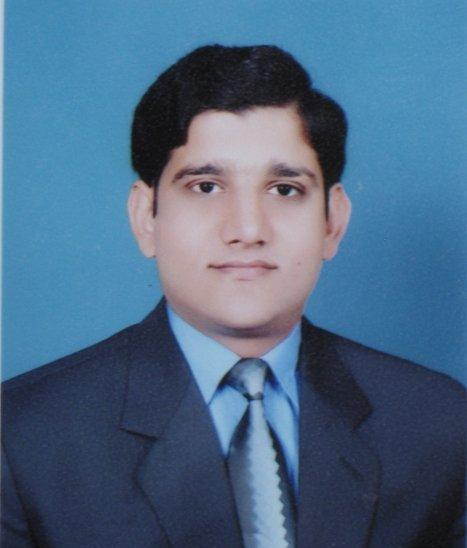
\includegraphics[width=0.50\textwidth]{back/about_the_author/about_the_author.jpg}
	\label{fig:about_the_author}
\end{figure}
\vspace{0.4in}
\normalfont
\end{center}
%% write text here

The author is member of Pasking Group. 
\end{document}

